\documentclass[11pt]{article}
\usepackage{fullpage}
\usepackage{verbatim}
\usepackage{moreverb}
\usepackage{amsmath}
\let\verbatiminput=\verbatimtabinput
\def\verbatimtabsize{4\relax}
\usepackage{tikz}
\usetikzlibrary{arrows,automata, positioning}
\usepackage{array}
\usepackage{booktabs}
\usepackage{minted}
\usepackage{parskip}
\usepackage{float}
\usepackage{pbox}
\usepackage{makecell}
\usepackage{gensymb}
\graphicspath{{images/}}
\usepackage{adjustbox}
\usepackage{color}
\definecolor{rltred}{rgb}{0.75,0,0}
\definecolor{rltgreen}{rgb}{0,0.5,0}
\definecolor{rltblue}{rgb}{0,0,0.75}

\usepackage[%pdftex,
    colorlinks=true,
    urlcolor=rltblue,               % \href{...}{...}
    anchorcolor=rltbrightblue,
    filecolor=rltgreen,             % \href*{...}
    linkcolor=rltred,               % \ref{...} and \pageref{...}
    menucolor=webdarkblue,
    citecolor=webbrightgreen,
    pagebackref,
    pdfpagemode=UseNone,
    bookmarksopen=true]{hyperref}
\usepackage{graphicx}
\usepackage{hyperref}

\newcommand{\instbit}[1]{\mbox{\scriptsize #1}}
\newcommand{\instbitrange}[2]{~\instbit{#1} \hfill \instbit{#2}~}

\newcommand{\currentSemester}{Spring 2020}
\newcommand{\projectSpecVersion}{4.4}

\newcommand{\dueDateTime}{end of week}

\newcommand{\blockDiagramTaskName}{Checkpoint 1}
\newcommand{\blockDiagramDueDate}{Mar 22, 2020}
\newcommand{\blockDiagramTimeAlloted}{1 week}

\newcommand{\ALUTaskName}{Checkpoint 1.1}
\newcommand{\ALUDueDate}{April 5, 2020}
\newcommand{\ALUTimeAlloted}{2 week}

\newcommand{\baseCPUTaskName}{Checkpoint 2}
\newcommand{\baseCPUDueDate}{April 12, 2020}
\newcommand{\baseCPUTimeAlloted}{1 weeks}

\newcommand{\imageTaskName}{Checkpoint 3}
\newcommand{\imageDueDate}{April 26, 2020}
\newcommand{\imageTimeAlloted}{2 weeks}

\newcommand{\optTaskName}{Checkpoint 4}
\newcommand{\optDueDate}{May 8, 2020}
\newcommand{\optTimeAlloted}{2 weeks}

\newcommand{\finalCheckoffDueDate}{May 8 (by appointment)}

\newcommand{\finalReportDueDate}{May 11}

\newcommand{\skeletonRepoName}{project\_skeleton\_sp20}
\newcommand{\semesterName}{sp20}

%Also, change the info in minted blocks.  This includes the "Setting up your Code Repository" section and the "Setting up the Vivado Project" section


\begin{document}
\begin{center}
{\bf
University of California at Berkeley \\
College of Engineering \\
Department of Electrical Engineering and Computer Science \\
}
\end{center}

\begin{center}
EECS151/251A - LB, \currentSemester
\end{center}

\begin{center}
\LARGE
{\bf Project Specification: RISCV151 }  \\
Version \projectSpecVersion
\end{center}

\tableofcontents

\newpage

\section{Introduction}
The goal of this project is to familiarize EECS151/251A students with the methods and tools of digital design.
Working alone or in a team of two, you will design and implement a 3-stage pipelined RISC-V CPU with a UART for tethering.
<<<<<<< HEAD
Afterwards, you will build a 2D Convolutional hardware accelerator and do a system integration with your RISC-V CPU.
=======
<<<<<<< HEAD
Afterwards, you will attach the IO circuits you built in the lab to the CPU, and design a 2D Convolutional filter accelerator for image processing applications.
=======
Afterwards, you will build a 2D Convolutional hardware accelerator and do a system integration with your RISC-V CPU.
>>>>>>> d876782f5951ebb67897a68d2a811cd9a1da2e96
>>>>>>> dev
Finally, you will optimize your CPU for performance (maximizing the Iron Law) and cost (FPGA resource utilization).

You will use Verilog to implement this system, targeting the Xilinx PYNQ platform (a PYNQ-Z1 development board with a Zynq 7000-series FPGA).
The project will give you experience designing with RTL descriptions, resolving hazards in a simple pipeline, building interfaces, and teach you how to approach system-level optimization.

In tackling these challenges, your first step will be to map the high level specification to a design which can be translated into a hardware implementation.
After that, you will produce and debug that implementation.
These first steps can take significant time if you have not thought out your design prior to trying implementation.

As in previous semesters, your EECS151/251A project is probably the largest project you have faced so far here at Berkeley.
Good time management and good design organization is critical to your success.

\subsection{Tentative Deadlines}
\label{tentative_deadlines}
The following is a brief description of each checkpoint and approximately how many weeks will be alloted to each one. Note that this schedule is tentative and is subjected to change as the semester progresses.

%The current schedule is summarised at the end of the document in Section \ref{project_timeline}.

\begin{itemize}

  \item \textbf{\blockDiagramDueDate \space - \blockDiagramTaskName \space (\blockDiagramTimeAlloted)} - Submit a report to Gradescope with the following items: a schematic of your processor's datapath and pipeline stages, and your answers to the checkpoint 1 questions. The TA will give you feedback if applicable. In addition, push all of your IO-circuit Verilog modules that you have implemented in the labs to your assigned Github repository: \verb|debouncer|, \verb|edge_detector|, \verb|synchronizer|, \verb|fifo|, \verb|uart_receiver|, \verb|uart_transmitter|, \verb|display_controller|.
  \item \textbf{\ALUDueDate \space - \ALUTaskName \space (\ALUTimeAlloted)} - Go over your RISC-V microarchitecture with the TA (via Zoom). You should have a working ALU module and a complete instructional decoder by this point, and some basic datapath and control logic. This is mainly for the TA to keep track of your current progress.
  \item \textbf{\baseCPUDueDate \space - \baseCPUTaskName \space (\baseCPUTimeAlloted)} - Implement a fully functional RISC-V processor core in Verilog. Your processor core should pass the assembly tests.
  \item \textbf{\imageDueDate \space - \imageTaskName \space (\imageTimeAlloted)} - Attach I/O components from lab to your processor (FIFOs, buttons, switches, display), and 2D Convolutional filter. If time permits, interfacing with off-chip DRAMs using AXI4 bus.

  \item \textbf{\blockDiagramDueDate \space - \blockDiagramTaskName \space (\blockDiagramTimeAlloted)} - Submit a report to Gradescope with the following items: a schematic of your processor's datapath and pipeline stages, and your answers to the checkpoint 1 questions. The TA will give you feedback if applicable. In addition, push all of your IO-circuit Verilog modules that you have implemented in the labs to your assigned Github repository: \verb|debouncer|, \verb|edge_detector|, \verb|synchronizer|, \verb|fifo|, \verb|uart_receiver|, \verb|uart_transmitter|.
  \item \textbf{\ALUDueDate \space - \ALUTaskName \space (\ALUTimeAlloted)} - You should have a working Riscv151 core that can decode and execute all RV32I instructions, including CSR. It is not required that your implementation is high-performance nor integrated with the UART modules.
  \item \textbf{\baseCPUDueDate \space - \baseCPUTaskName \space (\baseCPUTimeAlloted)} - Implement a fully functional RISC-V processor core in Verilog. Your processor core should pass the assembly tests.
<<<<<<< HEAD
<<<<<<< HEAD
  \item \textbf{\imageDueDate \space - \imageTaskName \space (\imageTimeAlloted)} - Attach I/O components from lab to your processor (FIFOs, buttons, switches), and \textbf{TBA}.
>>>>>>> 71cf8e2460eff1d217062926fce09ee05a5afbe9
=======
  \item \textbf{\imageDueDate \space - \imageTaskName \space (\imageTimeAlloted)} - Implement an IO memory-mapped hardware-accelerated 2D Convolutional filter.
>>>>>>> d876782f5951ebb67897a68d2a811cd9a1da2e96
=======
  

  \item \textbf{\imageDueDate \space - \imageTaskName \space (\imageTimeAlloted)} - Implement an IO memory-mapped hardware-accelerated 2D Convolutional filter.

>>>>>>> dev
  \item \textbf{\finalCheckoffDueDate \space - Final Checkoff + Demo} - Final processor optimization and checkoff
  \item \textbf{\finalReportDueDate \space - Project Report} - Final report due
\end{itemize}

\subsection{General Project Tips}
\label{tips}
Document your project as you go.
You should comment your Verilog and keep your diagrams up to date.
Aside from the final project report (you will need to turn in a report documenting your project), you can use your design documents to help the debugging process.

Finish the required features first.
Attempt extra features after everything works well.
\textbf{If your submitted project does not work by the final deadline, you will not get any credit for any extra credit features you have implemented.}

This project, as has been done in past semesters, will be divided into checkpoints. The following sections will specify the objectives for each checkpoint.

\section{Checkpoints 1 \& 2 - 3-stage Pipelined RISC-V CPU}
The first checkpoint in this project is designed to guide the development of a three-stage pipelined RISC-V CPU that will be used as a base system in subsequent checkpoints.

%\begin{figure}[hbt]
%\begin{center}
%  \includegraphics[width=0.7\textwidth]{sp20_overview.pdf}
%  \caption{High-level overview of the full system}
%  \label{fig:sys_overview}
%\end{center}
%\end{figure}

%The green (RISC-V core) block on the diagram is the focus of the first and second checkpoints.
%The third checkpoint will add audio and IO components in blue.
%Finally, the fourth checkpoint will implement the power management unit in red.

\subsection{Setting up your Code Repository}
The project skeleton files are available on Github.
The suggested way for initializing your repository with the skeleton files is as follows:

\begin{minted}[tabsize=2]{bash}
  git clone git@github.com:EECS150/project_skeleton_sp20.git
  cd project_skeleton_sp20
  git remote add my-repo git@github.com:EECS150/sp20_teamXX.git
  git push my-repo master
\end{minted}

Then reclone your repo and add the skeleton repo as a remote:
\begin{minted}[tabsize=2]{bash}
  cd ..
  rm -rf project_skeleton_sp20
  git clone git@github.com:EECS150/sp20_teamXX.git
  cd sp20_teamXX
  git remote add staff git@github.com:EECS150/project_skeleton_sp20.git
\end{minted}

To pull project updates from the skeleton repo, run \verb|git pull staff master|.

To get a team repo, fill the \href{https://docs.google.com/forms/d/1oBUvG6DH-QeFeeiaRB2vwItycJ2V-RA0Zt5n1dMdOco}{Google form} with your team information (names, Github logins). Only one person in a team is required to fill the form.

\textbf{You should check frequently for updates to the skeleton files.} Whenever you resume your work on the project,
it is highly suggested that you do git pull from the skeleton repo to get the latest update.
Update announcements will be posted to Piazza.

\subsection{Integrate Designs from Labs} \label{past_designs}
You should copy some modules you designed from the labs.
We suggest you keep these with the provided source files in \verb|hardware/src| (overwriting any provided skeletons).

\begin{minted}[tabsize=2]{bash}
  cd sp20_teamXX
  cp fpga_labs_sp20/lab6/debouncer.v sp20_teamXX/hardware/src/io_circuits/.
\end{minted}

\textbf{Copy these files from the labs:}
\begin{minted}{bash}
  lab6/debouncer.v
  lab6/synchronizer.v
  lab6/edge_detector.v
  lab6/fifo.v
  lab6/uart_receiver.v
  lab6/uart_transmitter.v
  lab6/display_controller.v
\end{minted}

\subsection{Project Skeleton Overview}
\begin{itemize}
  \item \texttt{hardware}
    \begin{itemize}
      \item \texttt{src}
        \begin{itemize}
          \item \texttt{z1top.v}: Top level module. The RISC-V CPU is instantiated here.
          \item \texttt{riscv\_core/Riscv151.v}: All of your CPU datapath and control should be contained in this file.
          \item \texttt{io\_circuits}: Your IO circuits from previous lab exercises.
          \item \texttt{EECS151.v}: Our EECS151-SP20 library file of register and memory modules. \textbf{You are expected to use these modules for your sequential logic}.
        \end{itemize}
      \item \texttt{sim}
        \begin{itemize}
          \item \verb|Riscv151_testbench.v|: Starting point for testing your CPU. The testbench checks if your CPU can execute the instruction correctly according to spec, and can handle several cases of hazards. You should make sure your CPU implementation pass this testbench before moving on.
          \item \verb|assembly_testbench.v|: The testbench works with the software in \texttt{software/assembly\_tests}.
          \item \verb|echo_testbench.v|: The testbench works with the software in \texttt{software/echo}. The CPU reads a character sent from the serial rx line and echoes it back to the serial tx line.
          \item \verb|isa_testbench.v|: The testbench works with the RISC-V ISA test suite in

\texttt{software/riscv-isa-tests}.

The testbench only runs one test at a time. To run multiple tests, use the script we provide (see \ref{riscv-isa-tests}).
        \end{itemize}
    \end{itemize}
  \item \texttt{software}
    \begin{itemize}
      \item \verb|bios151v3|: The BIOS program, which allows us to interact with our CPU via the UART. You need to compile it before creating a bitstream or running a simulation.
      \item \verb|echo|: The echo program, which emulates the FSM from Lab 5 in software.
      \item \verb|assembly_tests|: Use this as a template to write assembly tests for your processor designed to run in simulation.
      \item \verb|c_example|: Use this as an example to write C programs.
      \item \verb|riscv-isa-tests|: A comprehensive test suite for your CPU. Available after doing \verb|git submodule| (see \ref{riscv-isa-tests}).
      \item \verb|mmult|: This is a program to be run on the FPGA for Checkpoint 2. It generates 2 matrices and multiplies them. Then it returns a checksum to verify the correct result.
    \end{itemize}
\end{itemize}

To compile \texttt{software} go into a program directory and run \texttt{make}.
To build a bitstream run \texttt{make impl} in \texttt{hardware}.

\subsection{RISC-V 151 ISA}
Table \ref{tab:ISA} contains all of the instructions your processor is responsible for supporting.
It contains most of the instructions specified in the RV32I Base Instruction set, and allows us to maintain a relatively simple design while still being able to have a C compiler and write interesting programs to run on the processor.
For the specific details of each instruction, refer to sections 2.2 through 2.6 in the \href{http://riscv.org/specifications/}{RISC-V Instruction Set Manual}.

\subsubsection{CSR Instructions}
You will have to implement 2 CSR instructions to support running the standard RISC-V ISA test suite.
A CSR (or control status register) is some state that is stored independent of the register file and the memory.
While there are $2^{12}$ possible CSR addresses, you will only use one of them (\texttt{tohost = 0x51E}).
The \texttt{tohost} register is monitored by the RISC-V ISA testbench (\verb|isa_testbench.v|), and simulation ends when a non-zero value is written to this register.
A CSR value of 1 indicates success, and a value greater than 1 indicates which test failed.

There are 2 CSR related instructions that you will need to implement:
\begin{enumerate}
  \item \texttt{csrw tohost,x2}  (short for \texttt{csrrw x0,csr,rs1} where \texttt{csr = 0x51E})
  \item \texttt{csrwi tohost,1}  (short for \texttt{csrrwi x0,csr,uimm} where \texttt{csr = 0x51E})
\end{enumerate}

\texttt{csrw} will write the value from \texttt{rs1} into the addressed CSR.
\texttt{csrwi} will write the immediate (stored in the rs1 field in the instruction) into the addressed CSR.
Note that you do not need to write to \texttt{rd} (writing to x0 does nothing), since the CSR instructions are only used in simulation.

\begin{table}[p]
\caption{RISC-V ISA}
\label{tab:ISA}
\begin{small}
\begin{center}
\begin{tabular}{p{0in}p{0.4in}p{0.05in}p{0.05in}p{0.05in}p{0.05in}p{0.4in}p{0.6in}p{0.4in}p{0.6in}p{0.7in}l}
& & & & & & & & & & \\
                      &
\multicolumn{1}{l}{\instbit{31}} &
\multicolumn{1}{r}{\instbit{27}} &
\instbit{26} &
\instbit{25} &
\multicolumn{1}{l}{\instbit{24}} &
\multicolumn{1}{r}{\instbit{20}} &
\instbitrange{19}{15} &
\instbitrange{14}{12} &
\instbitrange{11}{7} &
\instbitrange{6}{0} \\
\cline{2-11}


&
\multicolumn{4}{|c|}{funct7} &
\multicolumn{2}{c|}{rs2} &
\multicolumn{1}{c|}{rs1} &
\multicolumn{1}{c|}{funct3} &
\multicolumn{1}{c|}{rd} &
\multicolumn{1}{c|}{opcode} & R-type \\
\cline{2-11}


&
\multicolumn{6}{|c|}{imm[11:0]} &
\multicolumn{1}{c|}{rs1} &
\multicolumn{1}{c|}{funct3} &
\multicolumn{1}{c|}{rd} &
\multicolumn{1}{c|}{opcode} & I-type \\
\cline{2-11}


&
\multicolumn{4}{|c|}{imm[11:5]} &
\multicolumn{2}{c|}{rs2} &
\multicolumn{1}{c|}{rs1} &
\multicolumn{1}{c|}{funct3} &
\multicolumn{1}{c|}{imm[4:0]} &
\multicolumn{1}{c|}{opcode} & S-type \\
\cline{2-11}


&
\multicolumn{4}{|c|}{imm[12$\vert$10:5]} &
\multicolumn{2}{c|}{rs2} &
\multicolumn{1}{c|}{rs1} &
\multicolumn{1}{c|}{funct3} &
\multicolumn{1}{c|}{imm[4:1$\vert$11]} &
\multicolumn{1}{c|}{opcode} & B-type \\
\cline{2-11}


&
\multicolumn{8}{|c|}{imm[31:12]} &
\multicolumn{1}{c|}{rd} &
\multicolumn{1}{c|}{opcode} & U-type \\
\cline{2-11}


&
\multicolumn{8}{|c|}{imm[20$\vert$10:1$\vert$11$\vert$19:12]} &
\multicolumn{1}{c|}{rd} &
\multicolumn{1}{c|}{opcode} & J-type \\
\cline{2-11}


&
\multicolumn{10}{c}{} & \\
&
\multicolumn{10}{c}{\bf RV32I Base Instruction Set} & \\
\cline{2-11}


&
\multicolumn{8}{|c|}{imm[31:12]} &
\multicolumn{1}{c|}{rd} &
\multicolumn{1}{c|}{0110111} & LUI \\
\cline{2-11}


&
\multicolumn{8}{|c|}{imm[31:12]} &
\multicolumn{1}{c|}{rd} &
\multicolumn{1}{c|}{0010111} & AUIPC \\
\cline{2-11}


&
\multicolumn{8}{|c|}{imm[20$\vert$10:1$\vert$11$\vert$19:12]} &
\multicolumn{1}{c|}{rd} &
\multicolumn{1}{c|}{1101111} & JAL \\
\cline{2-11}


&
\multicolumn{6}{|c|}{imm[11:0]} &
\multicolumn{1}{c|}{rs1} &
\multicolumn{1}{c|}{000} &
\multicolumn{1}{c|}{rd} &
\multicolumn{1}{c|}{1100111} & JALR \\
\cline{2-11}


&
\multicolumn{4}{|c|}{imm[12$\vert$10:5]} &
\multicolumn{2}{c|}{rs2} &
\multicolumn{1}{c|}{rs1} &
\multicolumn{1}{c|}{000} &
\multicolumn{1}{c|}{imm[4:1$\vert$11]} &
\multicolumn{1}{c|}{1100011} & BEQ \\
\cline{2-11}


&
\multicolumn{4}{|c|}{imm[12$\vert$10:5]} &
\multicolumn{2}{c|}{rs2} &
\multicolumn{1}{c|}{rs1} &
\multicolumn{1}{c|}{001} &
\multicolumn{1}{c|}{imm[4:1$\vert$11]} &
\multicolumn{1}{c|}{1100011} & BNE \\
\cline{2-11}


&
\multicolumn{4}{|c|}{imm[12$\vert$10:5]} &
\multicolumn{2}{c|}{rs2} &
\multicolumn{1}{c|}{rs1} &
\multicolumn{1}{c|}{100} &
\multicolumn{1}{c|}{imm[4:1$\vert$11]} &
\multicolumn{1}{c|}{1100011} & BLT \\
\cline{2-11}


&
\multicolumn{4}{|c|}{imm[12$\vert$10:5]} &
\multicolumn{2}{c|}{rs2} &
\multicolumn{1}{c|}{rs1} &
\multicolumn{1}{c|}{101} &
\multicolumn{1}{c|}{imm[4:1$\vert$11]} &
\multicolumn{1}{c|}{1100011} & BGE \\
\cline{2-11}


&
\multicolumn{4}{|c|}{imm[12$\vert$10:5]} &
\multicolumn{2}{c|}{rs2} &
\multicolumn{1}{c|}{rs1} &
\multicolumn{1}{c|}{110} &
\multicolumn{1}{c|}{imm[4:1$\vert$11]} &
\multicolumn{1}{c|}{1100011} & BLTU \\
\cline{2-11}


&
\multicolumn{4}{|c|}{imm[12$\vert$10:5]} &
\multicolumn{2}{c|}{rs2} &
\multicolumn{1}{c|}{rs1} &
\multicolumn{1}{c|}{111} &
\multicolumn{1}{c|}{imm[4:1$\vert$11]} &
\multicolumn{1}{c|}{1100011} & BGEU \\
\cline{2-11}


&
\multicolumn{6}{|c|}{imm[11:0]} &
\multicolumn{1}{c|}{rs1} &
\multicolumn{1}{c|}{000} &
\multicolumn{1}{c|}{rd} &
\multicolumn{1}{c|}{0000011} & LB \\
\cline{2-11}


&
\multicolumn{6}{|c|}{imm[11:0]} &
\multicolumn{1}{c|}{rs1} &
\multicolumn{1}{c|}{001} &
\multicolumn{1}{c|}{rd} &
\multicolumn{1}{c|}{0000011} & LH \\
\cline{2-11}


&
\multicolumn{6}{|c|}{imm[11:0]} &
\multicolumn{1}{c|}{rs1} &
\multicolumn{1}{c|}{010} &
\multicolumn{1}{c|}{rd} &
\multicolumn{1}{c|}{0000011} & LW \\
\cline{2-11}


&
\multicolumn{6}{|c|}{imm[11:0]} &
\multicolumn{1}{c|}{rs1} &
\multicolumn{1}{c|}{100} &
\multicolumn{1}{c|}{rd} &
\multicolumn{1}{c|}{0000011} & LBU \\
\cline{2-11}


&
\multicolumn{6}{|c|}{imm[11:0]} &
\multicolumn{1}{c|}{rs1} &
\multicolumn{1}{c|}{101} &
\multicolumn{1}{c|}{rd} &
\multicolumn{1}{c|}{0000011} & LHU \\
\cline{2-11}


&
\multicolumn{4}{|c|}{imm[11:5]} &
\multicolumn{2}{c|}{rs2} &
\multicolumn{1}{c|}{rs1} &
\multicolumn{1}{c|}{000} &
\multicolumn{1}{c|}{imm[4:0]} &
\multicolumn{1}{c|}{0100011} & SB \\
\cline{2-11}


&
\multicolumn{4}{|c|}{imm[11:5]} &
\multicolumn{2}{c|}{rs2} &
\multicolumn{1}{c|}{rs1} &
\multicolumn{1}{c|}{001} &
\multicolumn{1}{c|}{imm[4:0]} &
\multicolumn{1}{c|}{0100011} & SH \\
\cline{2-11}

&
\multicolumn{4}{|c|}{imm[11:5]} &
\multicolumn{2}{c|}{rs2} &
\multicolumn{1}{c|}{rs1} &
\multicolumn{1}{c|}{010} &
\multicolumn{1}{c|}{imm[4:0]} &
\multicolumn{1}{c|}{0100011} & SW \\
\cline{2-11}

&
\multicolumn{6}{|c|}{imm[11:0]} &
\multicolumn{1}{c|}{rs1} &
\multicolumn{1}{c|}{000} &
\multicolumn{1}{c|}{rd} &
\multicolumn{1}{c|}{0010011} & ADDI \\
\cline{2-11}

&
\multicolumn{6}{|c|}{imm[11:0]} &
\multicolumn{1}{c|}{rs1} &
\multicolumn{1}{c|}{010} &
\multicolumn{1}{c|}{rd} &
\multicolumn{1}{c|}{0010011} & SLTI \\
\cline{2-11}

&
\multicolumn{6}{|c|}{imm[11:0]} &
\multicolumn{1}{c|}{rs1} &
\multicolumn{1}{c|}{011} &
\multicolumn{1}{c|}{rd} &
\multicolumn{1}{c|}{0010011} & SLTIU \\
\cline{2-11}

&
\multicolumn{6}{|c|}{imm[11:0]} &
\multicolumn{1}{c|}{rs1} &
\multicolumn{1}{c|}{100} &
\multicolumn{1}{c|}{rd} &
\multicolumn{1}{c|}{0010011} & XORI \\
\cline{2-11}

&
\multicolumn{6}{|c|}{imm[11:0]} &
\multicolumn{1}{c|}{rs1} &
\multicolumn{1}{c|}{110} &
\multicolumn{1}{c|}{rd} &
\multicolumn{1}{c|}{0010011} & ORI \\
\cline{2-11}

&
\multicolumn{6}{|c|}{imm[11:0]} &
\multicolumn{1}{c|}{rs1} &
\multicolumn{1}{c|}{111} &
\multicolumn{1}{c|}{rd} &
\multicolumn{1}{c|}{0010011} & ANDI \\
\cline{2-11}

&
\multicolumn{4}{|c|}{0000000} &
\multicolumn{2}{c|}{shamt} &
\multicolumn{1}{c|}{rs1} &
\multicolumn{1}{c|}{001} &
\multicolumn{1}{c|}{rd} &
\multicolumn{1}{c|}{0010011} & SLLI \\
\cline{2-11}

&
\multicolumn{4}{|c|}{0000000} &
\multicolumn{2}{c|}{shamt} &
\multicolumn{1}{c|}{rs1} &
\multicolumn{1}{c|}{101} &
\multicolumn{1}{c|}{rd} &
\multicolumn{1}{c|}{0010011} & SRLI \\
\cline{2-11}

&
\multicolumn{4}{|c|}{0100000} &
\multicolumn{2}{c|}{shamt} &
\multicolumn{1}{c|}{rs1} &
\multicolumn{1}{c|}{101} &
\multicolumn{1}{c|}{rd} &
\multicolumn{1}{c|}{0010011} & SRAI \\
\cline{2-11}

&
\multicolumn{4}{|c|}{0000000} &
\multicolumn{2}{c|}{rs2} &
\multicolumn{1}{c|}{rs1} &
\multicolumn{1}{c|}{000} &
\multicolumn{1}{c|}{rd} &
\multicolumn{1}{c|}{0110011} & ADD \\
\cline{2-11}

&
\multicolumn{4}{|c|}{0100000} &
\multicolumn{2}{c|}{rs2} &
\multicolumn{1}{c|}{rs1} &
\multicolumn{1}{c|}{000} &
\multicolumn{1}{c|}{rd} &
\multicolumn{1}{c|}{0110011} & SUB \\
\cline{2-11}

&
\multicolumn{4}{|c|}{0000000} &
\multicolumn{2}{c|}{rs2} &
\multicolumn{1}{c|}{rs1} &
\multicolumn{1}{c|}{001} &
\multicolumn{1}{c|}{rd} &
\multicolumn{1}{c|}{0110011} & SLL \\
\cline{2-11}

&
\multicolumn{4}{|c|}{0000000} &
\multicolumn{2}{c|}{rs2} &
\multicolumn{1}{c|}{rs1} &
\multicolumn{1}{c|}{010} &
\multicolumn{1}{c|}{rd} &
\multicolumn{1}{c|}{0110011} & SLT \\
\cline{2-11}

&
\multicolumn{4}{|c|}{0000000} &
\multicolumn{2}{c|}{rs2} &
\multicolumn{1}{c|}{rs1} &
\multicolumn{1}{c|}{011} &
\multicolumn{1}{c|}{rd} &
\multicolumn{1}{c|}{0110011} & SLTU \\
\cline{2-11}

&
\multicolumn{4}{|c|}{0000000} &
\multicolumn{2}{c|}{rs2} &
\multicolumn{1}{c|}{rs1} &
\multicolumn{1}{c|}{100} &
\multicolumn{1}{c|}{rd} &
\multicolumn{1}{c|}{0110011} & XOR \\
\cline{2-11}

&
\multicolumn{4}{|c|}{0000000} &
\multicolumn{2}{c|}{rs2} &
\multicolumn{1}{c|}{rs1} &
\multicolumn{1}{c|}{101} &
\multicolumn{1}{c|}{rd} &
\multicolumn{1}{c|}{0110011} & SRL \\
\cline{2-11}

&
\multicolumn{4}{|c|}{0100000} &
\multicolumn{2}{c|}{rs2} &
\multicolumn{1}{c|}{rs1} &
\multicolumn{1}{c|}{101} &
\multicolumn{1}{c|}{rd} &
\multicolumn{1}{c|}{0110011} & SRA \\
\cline{2-11}

&
\multicolumn{4}{|c|}{0000000} &
\multicolumn{2}{c|}{rs2} &
\multicolumn{1}{c|}{rs1} &
\multicolumn{1}{c|}{110} &
\multicolumn{1}{c|}{rd} &
\multicolumn{1}{c|}{0110011} & OR \\
\cline{2-11}

&
\multicolumn{4}{|c|}{0000000} &
\multicolumn{2}{c|}{rs2} &
\multicolumn{1}{c|}{rs1} &
\multicolumn{1}{c|}{111} &
\multicolumn{1}{c|}{rd} &
\multicolumn{1}{c|}{0110011} & AND \\
\cline{2-11}

&
\multicolumn{10}{c}{} & \\
&
\multicolumn{10}{c}{\bf RV32/RV64 \emph{Zicsr} Standard Extension} & \\
\cline{2-11}

&
\multicolumn{6}{|c|}{csr} &
\multicolumn{1}{c|}{rs1} &
\multicolumn{1}{c|}{001} &
\multicolumn{1}{c|}{rd} &
\multicolumn{1}{c|}{1110011} & CSRRW \\
\cline{2-11}

&
\multicolumn{6}{|c|}{csr} &
\multicolumn{1}{c|}{uimm} &
\multicolumn{1}{c|}{101} &
\multicolumn{1}{c|}{rd} &
\multicolumn{1}{c|}{1110011} & CSRRWI \\
\cline{2-11}

\end{tabular}
\end{center}
\end{small}

\end{table}


\subsection{Pipelining}
Your CPU must implement this instruction set using a 3-stage pipeline.
The division of the datapath into three stages is left unspecified as it is an important design decision with significant performance implications.
We recommend that you begin the design process by considering which elements of the datapath are synchronous and in what order they need to be placed.
After determining the design blocks that require a clock edge, consider where to place asynchronous blocks to minimize the critical path.
The RAMs we are using for the data, instruction, and BIOS memories are both \textbf{synchronous} read and \textbf{synchronous} write.

\subsection{Hazards}
As you have learned in lecture, pipelines create hazards.
Your design will have to resolve both control and data hazards.
You must resolve data hazards by implementing forwarding whenever possible.
This means that you must forward data from your data memory instead of stalling your pipeline or injecting NOPs.
All data hazards can be resolved by forwarding in a three-stage pipeline.

You'll have to deal with the following types of hazards:
\begin{enumerate}
  \item \textbf{Read-after-write data hazards} Consider carefully how to handle instructions that depend on a preceding load instruction, as well as those that depend on a previous arithmetic instruction.
  \item \textbf{Control hazards} What do you do when you encounter a branch instruction, a jal (jump and link), or jalr (jump from register and link)?
    You will have to choose whether to predict branches as taken or not taken by default and kill instructions that weren't supposed to execute if needed.
    You can begin by resolving branches by stalling the pipeline, and when your processor is functional, move to naive branch prediction.
\end{enumerate}

\subsection{Register File}
\label{reg_file}
We have provided a register file module for you in \verb|EECS151.v|: \verb|REGFILE_1W2R|. The register file has two asynchronous-read ports and one synchronous-write port (positive edge).

\subsection{RAMs}
\label{ram_info}
In this project, we will be using some memory blocks defined in \verb|EECS151.v| to implement memories for the processor.
As you may recall in previous lab exercises, the memory blocks can be either synthesized to Block RAMs or LUTRAMs on FPGA.
For the project, our memory blocks will be mapped to Block RAMs. Therefore, read and write to memory are \textbf{synchronous}.

\subsubsection{Initialization}

For synthesis, the BIOS memory is initialized with the contents of the BIOS program, and the other memories are zeroed out.

For simulation, the provided testbenches initialize the BIOS memory with a program specified by the testbench (see \verb|sim/assembly_testbench.v|).

\subsubsection{Endianness + Addressing}
The instruction and data RAMs have 16384 32-bit rows, as such, they accept 14 bit addresses.
The RAMs are \textbf{word-addressed}; this means that every unique 14 bit address refers to one 32-bit row (word) of memory.

However, the memory addressing scheme of RISC-V is \textbf{byte-addressed}.
This means that every unique 32 bit address the processor computes (in the ALU) points to one 8-bit byte of memory.

We consider the bottom 16 bits of the computed address (from the ALU) when accessing the RAMs.
The top 14 bits are the word address (for indexing into one row of the block RAM), and the bottom two are the byte offset (for indexing to a particular byte in a 32 bit row).

\label{endianness}
\begin{figure}[H]
  \begin{center}
    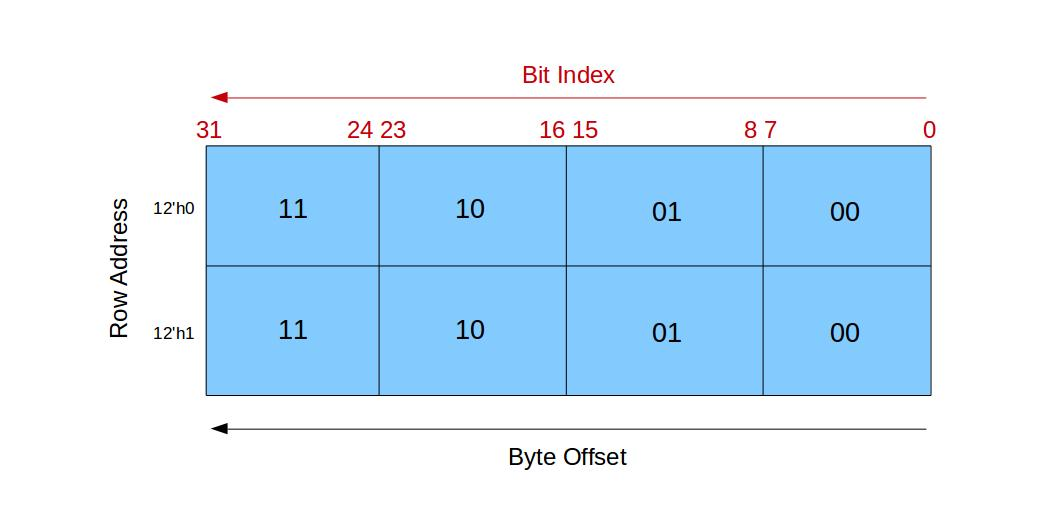
\includegraphics[width=0.6\textwidth]{endianness_img}
    \caption{Block RAM organization. The labels for row address \textbf{should read 14'h0 and 14'h1.}}
    \label{fig:endianness_img}
  \end{center}
\end{figure}

Figure \ref{fig:endianness_img} illustrates the 14-bit word addresses and the two bit byte offsets.
Observe that the RAM organization is \textbf{little-endian}, i.e. the most significant byte is at the most significant memory address (offset '11').

\subsubsection{Reading from RAMs}
Since the RAMs have 32-bit rows, you can only read data out of the RAM 32-bits at a time.
This is an issue when executing an \verb|lh| or \verb|lb| instruction, as there is no way to indicate which 8 or 16 of the 32 bits you want to read out.

Therefore, you will have to shift and mask the output of the RAM to select the appropriate portion of the 32-bits you read out.
For example, if you want to execute a \verb|lbu| on a byte address ending in \verb|2'b10|, you will only want bits \verb|[23:16]| of the 32 bits that you read out of the RAM (thus storing \verb|{24'b0, output[23:16]}| to a register).

\subsubsection{Writing to RAMs}
To take care of \verb|sb| and \verb|sh|, note that the \verb|we| input to the instruction and data memories is 4 bits wide.
These 4 bits are a byte mask telling the RAM which of the 4 bytes to actually write to.
If \verb|we|=\{4'b1111\}, then all 32 bits passed into the RAM would be written to the address given.

Here's an example of storing a single byte:
\begin{itemize}
  \item Write the byte \verb|0xa4| to address \verb|0x10000002| (byte offset = 2)
  \item Set \verb|we = {4'b0100}|
  \item Set \verb|din = {32'hxx_a4_xx_xx}| (\verb|x| means don't care)
\end{itemize}

\subsection{Memory Architecture}
The standard RISC pipeline is usually depicted with separate instruction and data memories.
Although this is an intuitive representation, it does not let us modify the instruction memory to run new programs.
Your CPU, by the end of this checkpoint, will be able to receive compiled RISC-V binaries though the UART, store them into instruction memory, then jump to the downloaded program.
To facilitate this, we will adopt a modified memory architecture shown in Figure \ref{fig:mem_arch}.

\begin{figure}[hbt]
  \begin{center}
    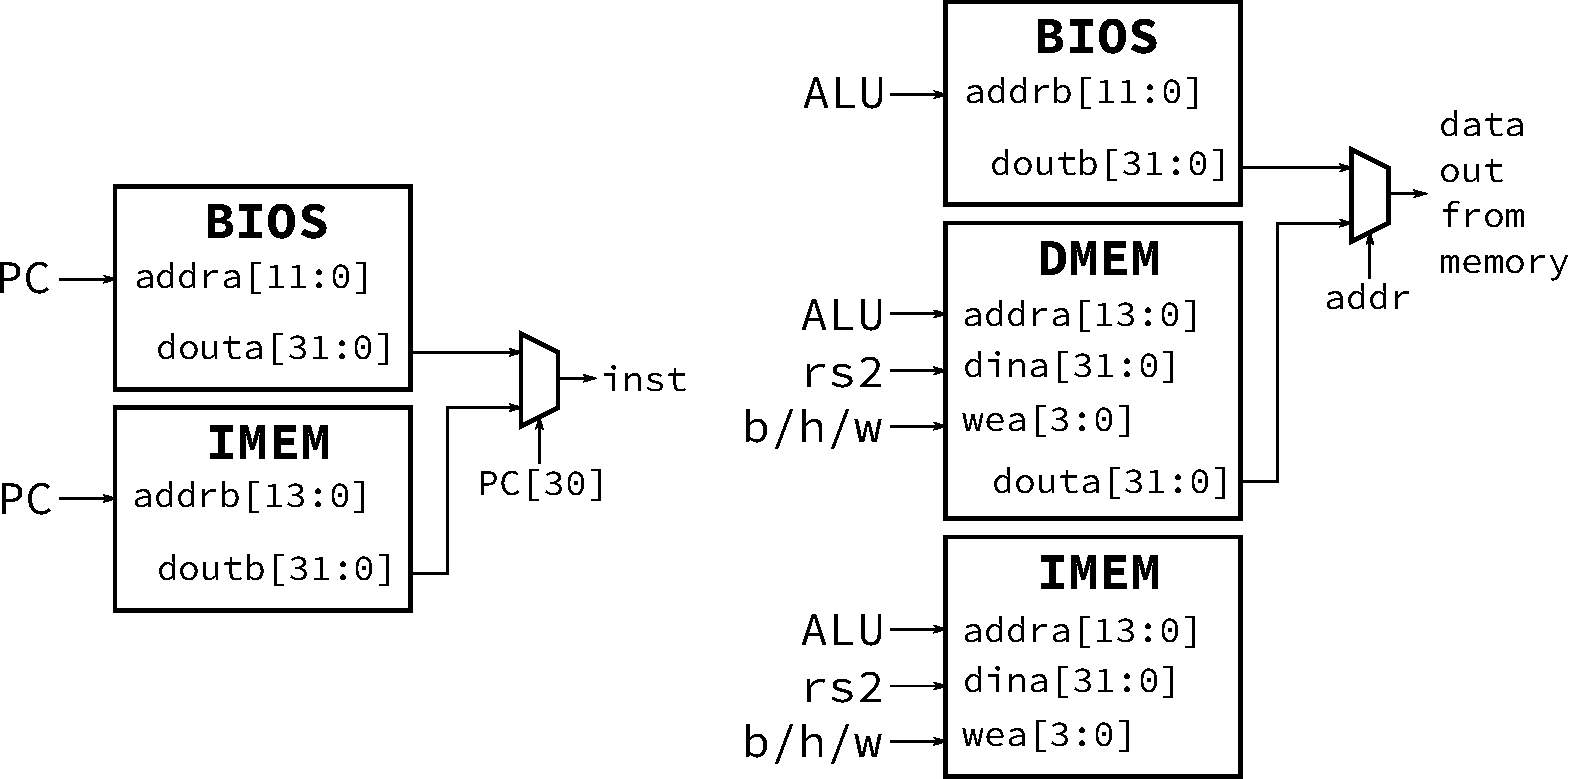
\includegraphics[width=0.8\textwidth]{memory_arch.pdf}
    \caption{The Riscv151 memory architecture. There is only 1 IMEM and DMEM instance in Riscv151 but their ports are shown separately in this figure for clarity. The left half of the figure shows the instruction fetch logic and the right half shows the memory load/store logic.}
    \label{fig:mem_arch}
  \end{center}
\end{figure}

\subsubsection{Summary of Memory Access Patterns}
The memory architecture will consist of three RAMs (instruction, data, and BIOS).
The RAMs are memory resources (block RAMs) contained within the FPGA chip, and no external (off-chip, DRAM) memory will be used for this project.

The processor will begin execution from the BIOS memory, which will be initialized with the BIOS program (in \verb|software/bios151v3|).
The BIOS program should be able to read from the BIOS memory (to fetch static data and instructions), and read and write the instruction and data memories.
This allows the BIOS program to receive user programs over the UART from the host PC and load them into instruction memory.

You can then instruct the BIOS program to jump to an instruction memory address, which begins execution of the program that you loaded.
At any time, you can press the reset button on the board to return your processor to the BIOS program.

\subsubsection{Unaligned Memory Accesses}
In the official RISC-V specification, unaligned loads and stores are supported.
However, in your project, you can ignore instructions that request an unaligned access.
Assume that the compiler will never generate unaligned accesses.

\subsubsection{Address Space Partitioning}
Your CPU will need to be able to access multiple sources for data as well as control the destination of store instructions.
In order to do this, we will partition the 32-bit address space into four regions: data memory read and writes, instruction memory writes, BIOS memory reads, and memory-mapped I/O.
This will be encoded in the top nibble (4 bits) of the memory address generated in load and store operations, as shown in Table \ref{mem_space1}.
In other words, the target memory/device of a load or store instruction is dependent on the address.
The reset signal should reset the PC to the value defined by the parameter \verb|RESET_PC| which is by default the base of BIOS memory (\verb|0x40000000|).

\begin{table}[hbt]
  \begin{center}
    \caption{Memory Address Partitions}
    \label{mem_space1}
    \begin{tabular}{l l l l l}
      \bottomrule
      \textbf{Address[31:28]} & \textbf{Address Type} & \textbf{Device} & \textbf{Access} & \textbf{Notes} \\
      \midrule
      4'b00x1 & Data & Data Memory & Read/Write &\\
      4'b0001 & PC  &  Instruction Memory & Read-only &\\
      4'b001x & Data & Instruction Memory & Write-Only & Only if PC[30] == 1'b1\\
      4'b0100 & PC  & BIOS Memory & Read-only &\\
      4'b0100 & Data & BIOS Memory & Read-only &\\
      4'b1000 & Data & I/O & Read/Write &\\
      \bottomrule
    \end{tabular}
  \end{center}
\end{table}

Each partition specified in Table \ref{mem_space1} should be enabled based on its associated bit in the address encoding.
This allows operations to be applied to multiple devices simultaneously, which will be used to maintain memory consistency between the data and instruction memory.

For example, a store to an address beginning with \verb|0x3| will write to both the instruction memory and data memory, while storing to addresses beginning with \verb|0x2| or \verb|0x1| will write to only the instruction or data memory, respectively.
For details about the BIOS and how to run programs on your CPU, see Section~\ref{bios_info}.

Please note that a given address could refer to a different memory depending on which address type it is.
For example the address \verb|0x10000000| refers to the data memory when it is a data address while a program counter value of \verb|0x10000000| refers to the instruction memory.

The note in the table above (referencing PC[30]), specifies that you can only write to instruction memory if you are currently executing in BIOS memory.
This prevents programs from being self-modifying, which would drastically complicate your processor.

\subsubsection{Memory Mapped I/O}
\label{mmio}
At this stage in the project the only way to interact with your CPU is through the UART.
The UART from Lab 5 accomplishes the low-level task of sending and receiving bits from the serial lines, but you will need a way for your CPU to send and receive bytes to and from the UART.
To accomplish this, we will use memory-mapped I/O, a technique in which registers of I/O devices are assigned memory addresses.
This enables load and store instructions to access the I/O devices as if they were memory.

To determine CPI (cycles per instruction) for a given program, the I/O memory map is also used to include instruction and cycle counters.

Table~\ref{mem_map1} shows the memory map for this stage of the project.

\begin{table}[hbt]
  \begin{center}
    \caption{I/O Memory Map}
    \label{mem_map1}
    \begin{adjustbox}{width=\columnwidth,center}
    \begin{tabular}{l l l l}
      \toprule
      \textbf{Address} & \textbf{Function} & \textbf{Access} & \textbf{Data Encoding}\\
      \midrule
      \verb|32'h80000000| & UART control & Read & \verb|{30'b0, uart_rx_data_out_valid, uart_tx_data_in_ready}| \\
      \verb|32'h80000004| & UART receiver data & Read & \verb|{24'b0, uart_rx_data_out}| \\
      \verb|32'h80000008| & UART transmitter data & Write & \verb|{24'b0, uart_tx_data_in}| \\
      \midrule
      \verb|32'h80000010| & Cycle counter & Read & Clock cycles elapsed \\
      \verb|32'h80000014| & Instruction counter & Read & Number of instructions executed \\
      \verb|32'h80000018| & Reset counters to 0 & Write & N/A \\
      \bottomrule
    \end{tabular}
    \end{adjustbox}
  \end{center}
\end{table}

You will need to determine how to translate the memory map into the proper ready-valid handshake signals for the UART.
Your UART should respond to \verb|sw, sh, and sb| for the transmitter data address, and should also respond to \verb|lw, lh, lb, lhu, and lbu| for the receiver data and control addresses.

You should treat I/O such as the UART just as you would treat the data memory.
This means that you should assert the equivalent write enable (i.e. valid) and data signals at the end of the execute stage, and read in data during the memory stage.
The CPU itself should not check the \verb|uart_rx_data_out_valid| and \verb|uart_tx_data_in_ready| signals; this check is handled in software.
The CPU needs to drive \verb|uart_rx_data_out_ready| and \verb|uart_tx_data_in_valid| correctly.

The cycle counter should be incremented every cycle, and the instruction counter should be incremented for every instruction that is committed (you should not count bubbles injected into the pipeline or instructions run during a branch mispredict).
From these counts, the CPI of the processor can be determined for a given benchmark program.

\subsection{Testing}
\label{testing}
The design specified for this project is a complex system and debugging can be very difficult without tests that increase visibility of certain areas of the design.
In assigning partial credit at the end for incomplete projects, we will look at testing as an indicator of progress.
A reasonable order in which to complete your testing is as follows:

\begin{enumerate}
  \item Test that your modules work in isolation via Verilog testbenches
  \item Test that your Riscv151 work with the \verb|Riscv151_testbench.v|
  \item Test the entire CPU one instruction at a time with hand-written assembly --- see \verb|assembly_testbench.v|
  \item Run the \verb|riscv-tests| ISA test suite
  \item Test the CPU's memory mapped I/O --- see \verb|echo_testbench.v|
\end{enumerate}

\subsection{Riscv151 Tests}

Once you are confident that the individual components of your processor are working in isolation, you will want to test the entire processor as a whole. One way to do this is to pass the \verb|Riscv151_testbench|. To run the test, use the following command:\\
\verb|make sim tb=Riscv151_testbench|

The testbench covers all RV32I instructions. To pass this testbench, you should have a working Riscv151 implementation that can decode and execute all the instructions in the spec, including CSR instructions. Several hazard cases are also tested. The testbench does not work with any software code as in the following sections, but rather it manually initializes the instructions and data in the memory blocks for each test. The testbench does not cover reading from BIOS memory nor memory mapped IO. You will need to complete these compoenents before moving on with other testbenches.

\subsection{Software Toolchain - Writing RISC-V Programs}
\label{toolchain}
A GCC RISC-V toolchain has been built and installed in the eecs151 home directory; these binaries will run on any of the c125m machines in the 125 Cory lab. The \href{https://berkeley.box.com/s/s4z0ykpf0tudrm9hce8fsmitpgb2khhe}{VM Image} also has the toolchain installed along with Vivado 2019.1.

The most relevant programs in the toolchain are:
\begin{itemize}
    \item \verb|riscv64-unknown-elf-gcc|: GCC for RISC-V, compiles C code to RISC-V binaries.
    \item \verb|riscv64-unknown-elf-as|: RISC-V assembler, compiles assembly code to RISC-V binaries.
    \item \verb|riscv64-unknown-elf-objdump|: Dumps RISC-V binaries as readable assembly code.
\end{itemize}

Look at the \verb|software/c_example| folder for an example of a C program.

There are several files:
\begin{itemize}
    \item \verb|start.s|: This is an assembly file that contains the start of the program.
      It initialises the stack pointer then jumps to the \verb|main| label.
      Edit this file to move the top of the stack.
      Typically your stack pointer is set to the top of the data memory address space, so that the stack has enough room to grow downwards.

    \item \verb|c_example.ld|: This linker script sets the base address of the program.
      For Checkpoint 2, this address should be in the format \verb|0x1000xxxx|
      The .text segment offset is typically set to the base of the instruction memory address space.

    \item \verb|c_example.elf|: Binary produced after running \verb|make|.\\Use \verb|riscv64-unknown-elf-objdump -Mnumeric -D c_example.elf| to view the assembly code.
    \item \verb|c_example.dump|: Assembly dump of the binary.
\end{itemize}

\subsection{Assembly Tests}
\label{assembly_tests}
Hand written assembly tests are in \verb|software/assembly_tests/start.s| and the corresponding testbench is in \verb|hardware/sim/assembly_testbench.v|.
To run the test, run:\\
\verb|make sim/assembly_testbench.fst| (iverilog) or \verb|make sim/assembly_testbench.vpd| (VCS).

If you want to forcibly re-run the test even though you didn't change the Verilog, run:\\
\verb|make -B sim/assembly_testbench.fst|

\verb|start.s| contains assembly that's compiled and loaded into the BIOS RAM by the testbench.
\begin{minted}[breaklines]{asm}
_start:

# Test ADD
li x10, 100         # Load argument 1 (rs1)
li x11, 200         # Load argument 2 (rs2)
add x1, x10, x11    # Execute the instruction being tested
li x20, 1           # Set the flag register to stop execution and inspect the result register
                    # Now we check that x1 contains 300 in the testbench

Done: j Done
\end{minted}

The \verb|assembly_testbench| toggles the clock one cycle at time and waits for register \verb|x20| to be written with a particular value (in the above example: 1).
Once \verb|x20| contains 1, the testbench inspects the value in \verb|x1| and checks it is 300, which indicates your processor correctly executed the add instruction.

If the testbench times out it means \verb|x20| never became 1, so the processor got stuck somewhere or \verb|x20| was written with another value.

You should add your own tests to verify that your processor can execute different instructions correctly. Modify the file \verb|start.s| to add your assembly code, then rerun the RTL simulation.

\subsection{RISC-V ISA Tests}\label{riscv-isa-tests}
You will need the CSR instructions to work before you can use this test suite, and you should have confidence in your hand-written assembly tests.
Test the CSR instructions using hand assembly tests.

To run the ISA tests, first pull the latest skeleton changes:
\begin{minted}{bash}
git pull staff master
git submodule update --init --recursive
\end{minted}

Then run

\begin{minted}{bash}
cd hardware
make sim tb=isa_testbench
\end{minted}

To run a particular ISA test (e.g. \verb|add|) run \verb|make sim tb=isa_testbench test=add|. The simulation should print out which tests passed or failed and their simulation cycles.

%To check what tests passed run \texttt{cat sim/isa/*.log | grep -i pass}.
%To check for failures run \texttt{cat sim/isa/*.log | grep -i fail}.

If you're failing other tests, debug using the test assembly file in\\\verb|software/riscv-isa-tests/riscv-tests/isa/rv32ui| or the generated assembly dump.

The \verb|RESET_PC| parameter is used in \verb|isa_testbench| to start the test in the IMEM instead of the BIOS.
Make sure you have used it in \verb|Riscv151.v|.

\subsection{Echo Test}

You should have your UART modules integrated with the CPU before running this test. The test verifies if your CPU is able to: check the UART status, read a character from UART Receiver, and write a character to UART Transmitter. Take a look at the software code \verb|software/echo/echo.c| to see what it does. The testbench loads the MIF file compiled from the software code, and load it to the BIOS memory in a similar manner to the assembly test and riscv-isa tests.

To run the echo test, run

\begin{minted}{bash}
make sim tb=echo_testbench
\end{minted}

The testbench, acts like a host, sends multiple characters via the serial line, then waits until it receives all the characters back. It is similar to how we test the UART Receiver and UART Transmitter module in Lab 6, but this time we test both of them along with your RISC-V CPU.

\subsection{BIOS and Programming your CPU}
\label{bios_info}

We have provided a BIOS program in \verb|software/bios151v3| that allows you to interact with your CPU and download other programs over UART.
The BIOS is just an infinite loop that reads from the UART, checks if the input string matches a known control sequence, and then performs an associated action.
For detailed information on the BIOS, see Appendix \ref{sec:biosinfo}.

To run the BIOS:
\begin{enumerate}
  \item Verify that the stack pointer and .text segment offset are set properly in \verb|start.s| and \verb|bios151v3.ld| in software/bios151v3 directory
  \item Build a bitstream and program the FPGA. Run \verb|make write-bitstream| in \verb|hardware|
  \item Use screen to access the serial port:
    \begin{minted}[tabsize=2]{bash}
    screen $SERIALTTY 115200
    \end{minted}
  \item Press the reset button to make the CPU PC go to the start of BIOS memory
\end{enumerate}

Close screen using \verb|Ctrl-a Shift-k|, or other students won't be able to use the serial port!
If you can't access the serial port you can run \verb|killscreen| to kill all screen sessions.

If all goes well, you should see a \verb|151 >| prompt after pressing return. The following commands are available:
\begin{itemize}
    \item \verb|jal <address>|: Jump to address (hex).
    \item \verb|sw, sb, sh <data> <address>|: Store data (hex) to address (hex).
    \item \verb|lw, lbu, lhu <address>|: Prints the data at the address (hex).
\end{itemize}

As an example, running \verb|sw cafef00d 10000000| should write to the data memory and running \verb|lw 10000000| should print the output \verb|10000000: cafef00d|.
Please also pay attention that writes to the instruction memory (\verb|sw ffffffff 20000000|) do not write to the data memory, i.e. \verb|lw 10000000| still should yield \verb|cafef00d|.

In addition to the command interface, the BIOS allows you to load programs to the CPU. \textit{With screen closed}, run:
\begin{minted}[tabsize=2]{bash}
    hex_to_serial <mif_file> <address>
\end{minted}

This stores the \verb|.mif| file at the specified hex address.
In order to write into both the data and instruction memories, \textbf{remember to set the top nibble to 0x3} (i.e. \verb|hex_to_serial echo.mif 30000000|, assuming the \verb|.ld| file sets the base address to \verb|0x10000000|).

You also need to ensure that the stack and base address are set properly (See Section \ref{toolchain}).
For example, before making the \verb|mmult| program you should set the set the base address to \verb|0x10000000| (see \ref{mmult}).
Therefore, when loading the \verb|mmult| program you should load it at the base address: \verb|hex_to_serial mmult.mif 30000000|.
Then, you can jump to the loaded \verb|mmult| program in in your screen session by using \verb|jal 10000000|.

\subsection{Target Clock Frequency}
By default, the CPU clock frequency is set at 50MHz.
It should be easy to meet timing at 50 MHz.
Look at the timing report to see if timing is met.
If you failed, the timing reports specify the critical path you should optimize.

For this checkpoint, we will allow you to demonstrate the CPU working at 50 MHz, but for the final checkoff at the end of the semester, you will need to optimize for a higher clock speed ($\geq$ 100MHz) for full credit.
Details on how to build your FPGA design with a different clock frequency will come later.

\subsection{Matrix Multiply}
\label{mmult}
To check the correctness and performance of your processor we have provided a benchmark in \verb|software/mmult/| which performs matrix multiplication.
You should be able to load it into your processor in the same way as loading the echo program.

This program computes $S=AB$, where $A$ and $B$ are 64$\times$64 matrices.
The program will print a checksum and the counters discussed in Section ~\ref{mmio}.
The correct checksum is \verb|0001f800|.
If you do not get this, there is likely a problem in your CPU with one of the instructions that is used by the BIOS but not mmult.

The matrix multiply program requires that the stack pointer and the offset of the .text segment be set properly, otherwise the program will not execute properly.

The stack pointer (set in \verb|start.s|) should start near the top of DMEM to avoid corrupting the program instructions and data.
It should be set to \verb|0x1000fff0| and the stack grows downwards.

The .text segment offset (set in \verb|mmult.ld|) needs to accommodate the full set of instructions and static data (three 64$\times$64 matrices) in the mmult binary.
It should be set to the base of DMEM: \verb|0x10000000|.

The program will also output the values of your instruction and cycle counters (in hex).
These can be used to calculate the CPI for this program.
Your target CPI should not be greater than 1.2.
If your CPI exceeds this value, you will need to modify your datapath and pipeline to reduce the number of bubbles inserted for resolving control hazards (since they are the only source of extra latency in our processor).
This might involve performing naive branch prediction or moving the jalr address calculation to an earlier stage.

\subsection{How to Survive This Checkpoint}
Start early and work on your design incrementally.
Draw up a very detailed and organised block diagram and keep it up to date as you begin writing Verilog.
Unit test independent modules such as the control unit, ALU, and regfile.
Write thorough and complex assembly tests by hand, and don't solely rely on the RISC-V ISA test suite.
The final BIOS program is several 1000 lines of assembly and will be nearly impossible to debug by just looking at the waveform.

The most valuable asset for this checkpoint will not be your GSIs but will be your fellow peers who you can compare notes with and discuss design aspects with in detail.
However, do NOT under any circumstances share source code.

Once you're tired, go home and \textit{sleep}. When you come back you will know how to solve your problem.

\subsubsection{How To Get Started}
It might seem overwhelming to implement all the functionality that your processor must support. The best way to implement your processor is in small increments, checking the correctness of your processor at each step along the way. Here is a guide that should help you plan out Checkpoint 1 and 2:

\begin{enumerate}
  \item \textit{Design.} You should start with a comprehensive and detailed design/schematic. Enumerate all the control signals that you will need. Be careful when designing the memory fetch stage since all the memories we use (BIOS, instruction, data, IO) are synchronous.
  \item \textit{First steps.} Implementing some modules that are easy to write and test.
  \item \textit{Control Unit + other small modules.} Implement the control unit, ALU, and any other small independent modules. Unit test them.
  \item \textit{Memory.} In the beginning, only use the BIOS memory in the instruction fetch stage and only use the data memory in the memory stage. This is enough to run assembly tests.
  \item \textit{Connect stages and pipeline.} Connect your modules together and pipeline them. At this point, you should be able to run integration tests using assembly tests for most R and I type instructions.
  \item \textit{Implement handling of control hazards.} Insert bubbles into your pipeline to resolve control hazards associated with JAL, JALR, and branch instructions. Don't worry about data hazard handling for now. Test that control instructions work properly with assembly tests.
  \item \textit{Implement data forwarding for data hazards.} Add forwarding muxes and forward the outputs of the ALU and memory stage. Remember that you might have to forward to ALU input A, ALU input B, and data to write to memory. Test forwarding aggressively; most of your bugs will come from incomplete or faulty forwarding logic. Test forwarding from memory and from the ALU, and with control instructions.
  \item \textit{Add BIOS memory reads.} Add the BIOS memory block RAM to the memory stage to be able to load data from the BIOS memory. Write assembly tests that contain some static data stored in the BIOS memory and verify that you can read that data.
  \item \textit{Add Inst memory writes and reads.} Add the instruction memory block RAM to the memory stage to be able to write data to it when executing inside the BIOS memory. Also add the instruction memory block RAM to the instruction fetch stage to be able to read instructions from the inst memory. Write tests that first write instructions to the instruction memory, and then jump (using jalr) to instruction memory to see that the right instructions are executed.
  \item \textit{Run Riscv151\_testbench}. The testbench verifies if your Riscv151 is able to read instructons from instruction memory block RAM, execute, and write data to either the Register File or data memory block RAM.
  \item \textit{Add cycle counters.} Begin to add the memory mapped IO components, by first adding the cycle and instruction counters. These are just 2 32-bit registers that your CPU should update on every cycle and every instruction respectively. Write tests to verify that your counters can be reset with a \verb|sw| instruction, and can be read from using a \verb|lw| instruction.
  \item \textit{Integrate UART.} Add the UART to the memory stage, in parallel with the data, instruction, and BIOS memories. Detect when an instruction is accessing the UART and route the data to the UART accordingly. Make sure that you are setting the UART ready/valid control signals properly as you are feeding or retrieving data from it. We have provided you with the \verb|echo_testbench| which performs a test of the UART.
  \item \textit{Run the BIOS.} If everything so far has gone well, program the FPGA. Verify that the BIOS performs as expected. As a precursor to this step, you might try to build a bitstream with the BIOS memory initialized with the echo program.
  \item \textit{Run matrix multiply.} Load the \verb|mmult| program with the \verb|hex_to_serial| utility, and run \verb|mmult| on the FPGA. Verify that it returns the correct checksum.
  \item \textit{Check CPI.} Compute the CPI when running the \verb|mmult| program. If you achieve a CPI 1.2 or smaller, that is acceptable, but if your CPI is larger than that, you should think of ways to reduce it.
\end{enumerate}

\subsection{Checkoff}
The checkoff is divided into two stages: block diagram/design and implementation.
The second part will require significantly more time and effort than the first one.
As such, completing the block diagram in time for the design review is crucial to your success in this project.

\subsubsection{\blockDiagramTaskName: Block Diagram}
The first checkpoint requires a detailed block diagram of your datapath.
The diagram should have a greater level of detail than a high level RISC datapath diagram.
You may complete this electronically or by hand.

If working by hand, we recommend working in pencil and combining several sheets of paper for a larger workspace.
If doing it electronically, you can use Inkscape, Google Drawings, draw.io or any program you want.

You should be able to describe in detail any smaller sub-blocks in your diagram.
Though the textbook diagrams are a decent starting place, remember that they often use asynchronous-read RAMs for the instruction and data memories, and we will be using synchronous-read block RAMs.

Additionally, you will be asked to provide short answers to the following questions based on how you structure your block diagram. The questions are intended to make you consider all possible cases that might happen when your processor execute instructions, such as data or control hazards. It might be a good idea to take a moment to think of the questions first, then draw your diagram to address them.

\begin{enumerate}
\item How many stages is the datapath you've drawn? (i.e. How many cycles does it take to execute 1 instruction?)
\item How do you handle ALU $\rightarrow$ ALU hazards?

addi x1, x2, 100

addi x2, x1, 100

\item How do you handle ALU $\rightarrow$ MEM hazards?

addi x1, x2, 100

sw x1, 0(x3)

\item How do you handle MEM $\rightarrow$ ALU hazards?

lw x1, 0(x3)

addi x1, x1, 100

\item How do you handle MEM $\rightarrow$ MEM hazards?

lw x1, 0(x2)

sw x1, 4(x2)

also consider:

lw x1, 0(x2)

sw x3, 0(x1)

\item Do you need special handling for 2 cycle apart hazards?

addi x1, x2, 100

 nop

 addi x1, x1, 100

\item How do you handle branch control hazards? (What is the mispredict latency, what prediction scheme are you using, are you just injecting NOPs until the branch is resolved, what about data hazards in the branch?)
\item How do you handle jump control hazards? Consider jal and jalr separately. What optimizations can be made to special-case handle jal? 
\item Can you handle jal writeback data forwarding?

jal x1, label

label: addi x2, x1, 4

\item How do you resolve JALR? How many NOPs are injected?
\item What is the most likely critical path in your design?
\item Where do the UART and cycle counters go? How are you going to drive data\_in\_valid (give a logic expression)?
\item Where does the BIOS mem go? How about the IMEM (in the memory stage)?
\end{enumerate}

Submit your block diagram and answers to Gradescope by \blockDiagramDueDate. If you are working in team, only one of you is required to upload the report. Please also remember to push your working IO circuits to your Github repository: the TA will test your circuits. The TA will also provide feedback for your block diagram proposal if applicable.

\subsubsection{\ALUTaskName: Riscv151 Test}
This checkpoint is for TA to keep track of your current progress, and to ensure that your implementation is on the right track. You are expected to have a fully-functioning Riscv151 core without IO blocks that passes the \verb|Riscv151_testbench.v|. You will also need to run Synthesis and Implementation to get the reports of area utilization and timing information of your design. This early-stage evaluation will give you some insight on how to further optimize your design to meet the spec requirement in future checkpoints. Although highly encouraged, it is not required to pass any software-related tests for this checkpoint, such as assembly tests or RISC-V test suite or echo. It is also not mandatory that you meet the target clock frequency at this checkpoint (50 MHz). The UART integration is also not required.

\subsubsection{\baseCPUTaskName: Base RISCV151 System}
This checkpoint requires a fully functioning three stage RISC-V CPU as described in this specification.
Checkoff will consist of a demonstration of the BIOS functionality, loading a program (\verb|echo| and \verb|mmult|) over the UART, and successfully jumping to and executing the program.

\textbf{\baseCPUTaskName \space materials should be committed to your project repository by \baseCPUDueDate.}

\subsubsection{Checkpoints 1 \& 2 Deliverables Summary}
\begin{center}
  \begin{tabular}{m{30mm} m{35mm} m{70mm}}
    \toprule
    \textbf{Deliverable} & \textbf{Due Date} & \textbf{Description} \\
    \midrule
    Block Diagram, RISC-V ISA Questions, IO code & \blockDiagramDueDate & Submit your diagram and answers to Gradescope. Push your IO code to your Github repository.\\
    \midrule
    Riscv151 testbench & \ALUDueDate \linebreak Check in code to Github & Pass the Riscv151 testbench. Submit the area and timing report of your design.\\
    \midrule
    RISC-V CPU & \baseCPUDueDate \linebreak Check in code to Github & Demonstrate that the BIOS works, you can use \verb|hex_to_serial| to load the \verb|echo| program, \verb|jal| to it from the BIOS, and have that program successfully execute. Load the mmult program with \verb|hex_to_serial|, \verb|jal| to it, and have it execute successfully and return the benchmarking results and correct checksum. Your CPI should not be greater than 1.2\\
    \bottomrule
  \end{tabular}
\end{center}

\pagebreak

\section{Checkpoint 3 - Hardware-accelerated 2D Convolutional Engine}

For this checkpoint, you are tasked with designing an efficient, parameterized 2D Convolutional hardware generator. You will be comparing the performance of your generator against the conv2D software code running on your RISC-V processor in Checkpoint 2.

Here are the new files added to this checkpoint:

\begin{itemize}
\item \verb|hardware/src/accelerator/conv2D_naive.v|: A naive conv2D hardware implementation.
\item \verb|hardware/src/accelerator/conv2D_mem_if.v|: A memory interface module of \texttt{conv2D\_naive}.
\item \verb|hardware/src/accelerator/conv2D_compute.v|: A compute module of \texttt{conv2D\_naive}.
\item \verb|hardware/src/accelerator/conv2D_opt.v|: A skeleton code for optimized conv2D hardware generator. Your task is to complete this file.
\item \verb|hardware/src/accelerator/io_dmem_controller.v|: A memory controller for interfacing conv2D accelerator and CPU Data memory.
\item \verb|hardware/sim/conv2D_testbench.v|: A standalone testbench that tests conv2D implementation.
\item \verb|software/conv2D/*|: Software files for conv2D that can be compiled to run on the Riscv151 processor in a similar manner to \texttt{mmult} of Checkpoint 2.
\end{itemize}

\subsection{2D Convolutional Operation}

2D Convolution is prevalent in many domains, ranging from signal and image processing to deep learning. An input matrix is convolved with a kernel, or weight matrix in a sliding window fashion to produce an output matrix. We refer to the input matrix as input feature map, and output matrix as output feature map. For simplicity, our conv2D implementation only supports square matrices for both feature map and weight data. In addition, the sliding window stride is always 1 and we pad zeros to the boundary of the input feature map. The supported datatype is 32-bit integer. The feature map dimension is a power-of-two value, and the weight dimension is an odd number.

Let's look at the software C code of a typical 2D convolutional operation.

\begin{minted}{C}
for (y = 0; y < FM_DIM; y = y + 1) {
  for (x = 0; x < FM_DIM; x = x + 1) {
    for (m = 0; m < WT_DIM; m = m + 1) {
      for (n = 0; n < WT_DIM; n = n + 1) {
        idx = x - WT_DIM / 2 + n;
        idy = y - WT_DIM / 2 + m;
        // Check for halo cells
        if (idx < 0 || idx >= FM_DIM || idy < 0 || idy >= FM_DIM)
          d = 0;
        else
          d = ifm_data[idy * FM_DIM + idx];

        ofm_sw_data[y * FM_DIM + x] = ofm_sw_data[y * FM_DIM + x] +
                                      d * weight_data[m * WT_DIM + n];
      }
    }
  }
}
\end{minted}

The code contains many levels of nested for loops. The outermost loops (y, x) iterate over each element of the output feature map, and the innermost loops (m, n) step through the weights to perform a dot product with a current sliding window of an input feature map. The input feature map array, output feature map array, and weight array are all stored in the data memory \texttt{DMem}. Additional check is required for halo cells (beyond the input matrix's boundary).

From the previous lab and homework execises, you already had some practice on mapping an algorithmic description of a problem (e.g., loop form) into a circuit implementation. This checkpoint brings it to another level by adding more complexity in terms of the number of loop levels and the amount of operations needed to carry out per loop iteration. How do we make sense between a software loop iteration and a hardware cycle? Would it be possible to map one or more software loop iterations to one hardware cycle? Can we overlap the operations of current loop iteration with the next one?

A straight mapping from the software description to hardware implementation, without considering many inherent characteristics of the system (memory latency, buffering, available compute blocks, etc.), gives poor result. Have a look at the baseline conv2D code given to you: \verb|hardware/src/accelerator/conv2D_naive.v|. This implementation reads the elements of input feature map redundantly without considering the fact that there are some overlap between the current and the next sliding window (with a stride of 1). Therefore, the memory latency quickly overwhelms the performance and leaves the compute unit starved for data. To build an efficient accelerator, one needs to not only understand how the software code works, but also be able to transform it to some form that is hardware-friendly in terms of memory access pattern, data reuse, and parallel execution units.

\subsection{IO Data Memory interface}

Our conv2D accelerator needs to read and write data to \texttt{DMem}. It adopts an interface similar to the AXI4 bus protocol, though much simpler. Separate read and write request and response channels are included. For each channel, a handshake mechanism (Ready/Valid) to used to indicate a successful transaction.

\textbf{1. Read Address Request channel}
\begin{itemize}
\item \textbf{req\_read\_addr}: Memory read request address (output)
\item \textbf{req\_read\_addr\_valid}: Memory read request address valid signal (output)
\item \textbf{req\_read\_addr\_ready}: Memory read request address ready signal (input)
\item \textbf{req\_read\_len}: Memory read burst length (output)
\end{itemize}

\textbf{2. Read Data Response channel}
\begin{itemize}
\item \textbf{resp\_read\_data}: Memory read response data (input)
\item \textbf{resp\_read\_data\_valid}: Memory read response data valid signal (input)
\item \textbf{resp\_read\_data\_ready}: Memory read response data ready signal (output)
\end{itemize}

\textbf{3. Write Address Request channel}
\begin{itemize}
\item \textbf{req\_write\_addr}: Memory write request address (output)
\item \textbf{req\_write\_addr\_valid}: Memory write request address valid signal (output)
\item \textbf{req\_write\_addr\_signal}: Memory write request address ready signal (output)
\item \textbf{req\_write\_len}: Memory write burst length (output)
\end{itemize}

\textbf{4. Write Data Request channel}
\begin{itemize}
\item \textbf{req\_write\_data}: Memory write request data (output)
\item \textbf{req\_write\_data\_valid}: Memory write request data valid (output)
\item \textbf{req\_write\_data\_ready}: Memory write request data ready (input)
\end{itemize}

\textbf{5. Write Status Response channel}
\begin{itemize}
\item \textbf{resp\_write\_status}: Memory write response status (input). 1 indicates a write sucess, 0 indicates a write failure
\item \textbf{resp\_write\_status\_valid}: Memory write response status valid signal (input)
\item \textbf{resp\_write\_status\_ready}: Memory write response status ready signal (output)
\end{itemize}

The memory signals connect to an \texttt{IO-DMem} controller (\verb|hardware/src/accelerator/io_dmem_controller.v|). A control logic in the controller converts the memory interfaces to the Block RAM interfaces of \texttt{DMem}. To enable read and write to DMem in parallel, we will use a dual-ported memory template for \texttt{DMem}. Port a is for IO read and \texttt{Riscv151}'s access, and port b is for IO write.

The memory interface supports burst transaction. For instances, if a burst length of 8 is set for read request at the address 10, the \texttt{IO-DMem} controller returns 8 data items from \texttt{DMem} of address 10, 11, 12, 13, 14, 15, 16, and 17, as shown in Figure \ref{fig:read_burst8}. Similar to write in Figure \ref{fig:write_burst8}. This is useful in the situation where the accelerator knows that it needs multiple items in row. A burst length of 1 means no burst mode. Note that, for a successful completion of one burst item (beat) transaction, both the ready and valid signals of read response data channel (or write request data channel) must be HIGH.

\begin{figure}[hbt]
\begin{center}
  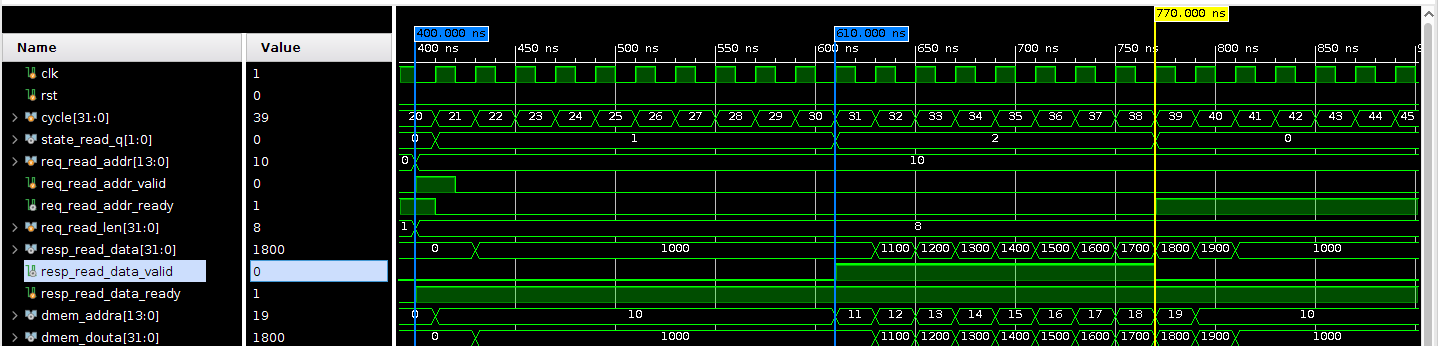
\includegraphics[width=1.0\textwidth]{read_burst8.png}
  \caption{A waveform of memory read with a burst length of 8 beats. Note that \textbf{resp\_read\_data\_valid} and \textbf{resp\_read\_data\_ready} must be high for one complete read beat.}
  \label{fig:read_burst8}
\end{center}
\end{figure}

\begin{figure}[hbt]
\begin{center}
  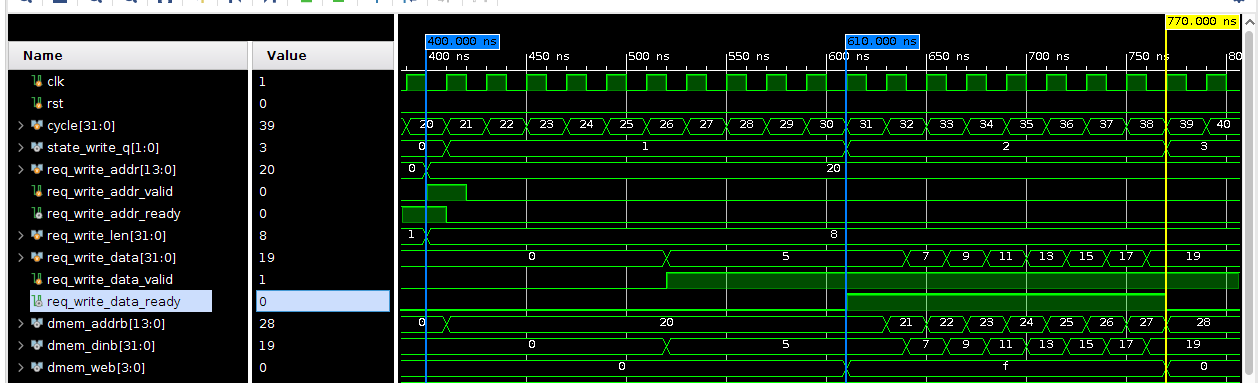
\includegraphics[width=1.0\textwidth]{write_burst8.png}
  \caption{A waveform of memory write with a burst length of 8 beats. Note that \textbf{req\_write\_data\_valid} and \textbf{req\_write\_data\_ready} must be high for one complete write beat.}
  \label{fig:write_burst8}
\end{center}
\end{figure}

Also note that our accelerator uses word-level addressing scheme, as oppose to byte-level addressing in RISC-V architecture. A memory read (write) retrieves (update) a full word of \texttt{DMem}.

In addition, reading and writing to \texttt{IO-DMem} incurs some latency. The latency (configurable in \verb|io_dmem_controller.v|) mimics the real setting where accessing to external memory is expensive, and one would need to think of a strategy to minimize the number of memory accesses to optimize performance. The IO latency is set to 10 cycles for both read and write.

\subsection{IO Memory-mapped addresses}

You will need to extend your IO memory-mapped logic to integrate the conv2D accelerator to Riscv151. We will use the load and store instructions to the memory-mapped addresses as a mechanism to control (start, reset) or check the status of conv2D (idle, done). To reset the accelerator, we use the same IO address as counters reset. In addition, we set the memory offsets of weight, input/output feature map arrays so that conv2D knows where to access (read/write) the correct data in \texttt{DMem}. This is a neat trick to avoid hard-coding the addresses or recompiling the whole bitstream everytime we change the memory layout of the arrays. The feature map dimension can also be set in software code. Our conv2D accelerator does not depend on any specific feature map dimension, but weight dimension. See the sofware code \verb|software/conv2D/conv2D.c| for the details of setting up various conv2D parameters in software.

\begin{table}[hbt]
  \begin{center}
    \caption{I/O Memory Map for conv2D}
    \label{mem_map_conv2D}
    \begin{adjustbox}{width=\columnwidth,center}
    \begin{tabular}{l l l l}
      \toprule
      \textbf{Address} & \textbf{Function} & \textbf{Access} & \textbf{Data Encoding}\\
      \midrule
      \verb|32'h80000018| & conv2D control (reset) & Write & N/A \\
      \verb|32'h80000040| & conv2D control (start) & Write & N/A \\
      \verb|32'h80000044| & conv2D status & Read & \verb|{30'b0, idle, done}| \\
      \verb|32'h80000048| & conv2D feature map dimension & Write & IO store data (32-bit) \\
      \verb|32'h8000004c| & conv2D weight offset & Write & IO store data (32-bit) \\
      \verb|32'h80000050| & conv2D input feature map offset & Write & IO store data (32-bit) \\
      \verb|32'h80000054| & conv2D output feature map offset & Write & IO store data (32-bit) \\
      \bottomrule
    \end{tabular}
    \end{adjustbox}
  \end{center}
\end{table}

\subsection{System integration}

Figure \ref{fig:system_integration} shows the big picture of the full system. A conv2D accelerator is an IO device that communicates with the Riscv151 processor via the IO bus. The Riscv151 ignites the accelerator and checks its status by means of IO memory-mapped memory instructions as similar to the UART modules. The \texttt{IO\_Dmem} controller services the memory requests and responses to the conv2D accelerator, and directly read/write to the Riscv151's data memory \texttt{DMem}. The \texttt{IO\_DMem} controller purposefully adds extra latency on a single read and write request to emulate off-chip IO latency.

\begin{figure}[hbt]
\begin{center}
  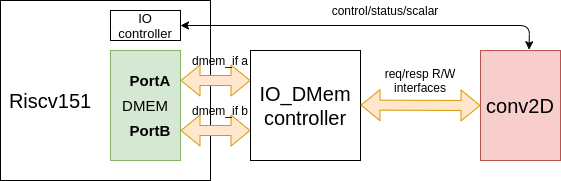
\includegraphics[width=0.5\textwidth]{Riscv151_conv2D.png}
  \caption{A full system of Riscv151 core + conv2D accelerator + IO\_DMem controller}
  \label{fig:system_integration}
\end{center}
\end{figure}

You might already notice that this system would not work with the current setting of Riscv151 in that \texttt{DMem} is a single-port memory block. In addition, port a is currently being used for the CPU load and store instructions. We would need to change two things to integrate the conv2D accelerator safely to the existing system.

\begin{itemize}
\item Use a dual-port memory template for \texttt{DMem} (look at \texttt{IMem} as an example)
\item Mux the address of \texttt{DMem}'s port a with the address generated from the \texttt{ALU} and the \texttt{IO\_DMem} controller (read request). The former is selected iif the conv2D accelerator is not running
\end{itemize}

This approach works if the CPU just spins doing nothing to wait for conv2D to be done. Another potential better approach is that the accelerator generates a stall signal to the CPU whenever it needs to read from \texttt{DMem}. To keep things simple, we will not take this road. Another pertaining issue is memory coherency due to memory writes from the accelerator and the CPU -- which is also beyond the scope of our project.

\subsection{Conv2D Streaming Engine}

Figure \ref{fig:conv2D_stream} demonstrates a streaming architectural engine that convolves the input feature map matrix with a 3x3 weight matrix. FIFOs are used to buffer temporary input and output items. Initially, the accelerator is pre-loaded with the weight data from the memory interface (not shown here) into the internal registers of the Processing Elements (PEs). Each PE performs a 1D convolution with its own set of weight elements and enqueues the result to a FIFO. A shift register is used to hold input feature map elements in a sliding window fashion. For a detailed cycle-by-cycle explanation of how the engine works, refer to the slides \href{https://drive.google.com/file/d/1QGFzt3gZ53IK1ZCIaJ57NUKucU77Nwd-}{\textbf{here}}.

The advantage of this architectural execution is the input (output) can be streamed sequentially, starting from the first to the last element, from the memory interface, if the input (output) feature map is stored in a contiguous region in the memory. This simplifies the logic regarding read/write to specific memory addresses for input (output) as in the naive implementation. If the memory interface supports burst mode, one can set the burst size to be the feature map size. Virtually, only one memory request for read and write is needed for such computation. Once there is a data item enqueued in an input FIFO buffer, the engine starts the computation. Since the engine is fully pipelined with an initial interval of 1, the total number of cycles required to complete the convolutional operation should be roughly equal to the padded feature map size with a few extra cycles due to initial IO overhead of read request and write request.

\begin{figure}[hbt]
\begin{center}
  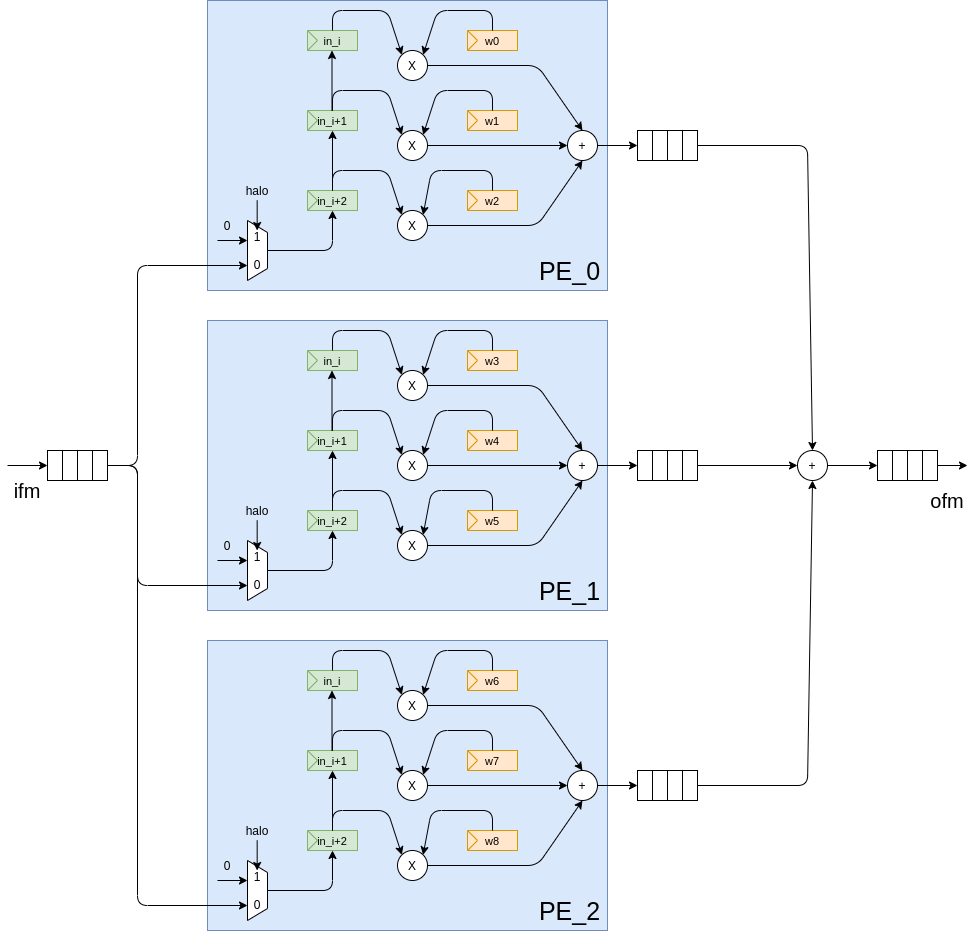
\includegraphics[width=0.8\textwidth]{conv2D_stream.png}
  \caption{Conv2D streaming dataflow engine for 3x3 weight matrix}
  \label{fig:conv2D_stream}
\end{center}
\end{figure}

As a suggestion, you can follow the block diagram to build your conv2D accelerator. You can make your own modifications to the suggested architecture, for example, by inserting additional registers to each PE to improve timing. Nonetheless, you are also welcomed to pursue your own ideas of building an efficient conv2D accelerator.

\subsection{Steps to complete Checkpoint 3}

First, run the RTL simulation of the given \texttt{conv2D\_naive} implementation with the testbench file \verb|hardware/sim/conv2D_testbench.v| to verify that it passes the testbench. The code requires a FIFO; make sure you have added your FIFO module to your repository (under \verb|hardware/src/io_circuits|). Note the number of simulation cycles it takes to finish conv2D.

\begin{minted}{bash}
cd hardware
make sim tb=conv2D_testbench
\end{minted}

The testbench does not invoke any software MIF file nor the RISC-V core that you designed in Checkpoint 2. Rather, it tests the functionality of the conv2D accelerator with \texttt{IO\_DMem} controller in place. A memory block is used to initialize data for testing. You may want to use the testbench when you design your own conv2D.

Once you confirm that the given code passes the simulation, the next step is integrating \texttt{conv2D\_naive} to your existing Riscv151 processor, along with \texttt{io\_dmem} controller. You need to expand your IO memory-mapped logic to perform load/store to the memory addresses of conv2D as mentioned in the section above, so that the CPU can control the conv2D accelerator from software. In addition, you will also need to convert \texttt{DMem} to dual-port memory block. Use \texttt{port a} for reading from \texttt{DMem}, and \texttt{port b} for writing to \texttt{DMem} from \texttt{IO\_DMem} controller. Don't forget to use the counters reset signal along with system reset to reset your conv2D module.

Next, generate a bitstream to configure your FPGA. Run the conv2D software program using the same command as in \texttt{mmult} case. Alternatively, you can do

\begin{minted}{bash}
cd software/conv2D
make run
\end{minted}

This will load the conv2D MIF file to the FPGA over UART. Do \texttt{jal 10000000} to begin the program execution. You should expect to see a correct checksum of \textbf{0000\_103e} for both hardware version (the conv2D accelerator) and the software version (the Riscv151 core). The cycle count of hardware execution is \textbf{17c1} which is 6081 cycles. This number should be roughly similar to the number of simulation cycles that you had observed before. In addition, there should not be any mismatches between the output feature map arrays of hardware and software execution.

Once you get a sense of how the entire flow works, it's time to code your own conv2D accelerator! You can use the naive code as a starting point, but please feel free to write your own code for everything. Add your own conv2D implementation to the file \verb|conv2D_opt.v|, then replace the naive module with the opt module for system integration. You should write a parameterizable weight-dimension conv2D generator. Once you verify that your accelerator works in simulation (with different feature map dimensions and weight dimensions), test it on the FPGA using the flow described above. Note the speedup over your Riscv151 processor in terms of \textbf{Cycle Count}.

\subsection{Checkpoint 3 Deliverables}

By \textbf{Sunday May 3, 2020, 11.59PM}, please have the following items submitted to Piazza as a private note to the TA to check off.

\begin{itemize}
\item A commit ID of your fully working Riscv151 + conv2D\_opt system.
\item Screenshot(s) to demonstrate that your bitstream correctly run the conv2D program with different feature map dimensions and weight dimensions on an FPGA. In particular, please test your implementation with the following parameters:

(LOG2\_FM\_DIM, WT\_DIM) = (3, 3), (4, 3), (5, 3), (6, 3),
                           (3, 5), (4, 5), (5, 5), (6, 5)

Note that you don't have to generate a new bitstream if you only change the feature map dimension; you just need to update the software C code and recompile it to generate a new MIF file to load to the FPGA. Please also report the speedup in each case.

\item Where do you think the speedup comes from? What makes the software (CPU) execution so inefficient in comparison to specialized hardware architecture?
\item The RV32I that our Riscv151 supports does not have a multiply instruction. Therefore, a multiplication is carried out by a software routine instead (look at the \textbf{times} function). If you could add a multiply instruction to your CPU to compute a multiplication in one cycle, analytically how much would the speedup be (for the case of (6, 3))?
\item Can you come up with an approach to implement a multiplication for your processor (that should be more efficient than invoking \textbf{times} function)? You don't have to implement it, just briefly describe how you would do it and how many cycles it would take.
\item What is the maximum achievable frequency of your system if conv2D is configured with a weight dimension of 3 (WT\_DIM=3)? What about the case of WT\_DIM=5?
\end{itemize} 

\newpage
\section{Final Checkpoint - Optimization}
This optimization checkpoint is lumped with the final checkoff.
This part of the project is designed to give students freedom to implement the optimizations of their choosing to improve the performance of their processor.

The optimization goal for this project is to minimize the \textbf{execution time} on the \verb|mmult| program, as defined by the 'Iron Law' of Processor Performance.

\begin{equation*}
\frac{\text{Time}}{\text{Program}} = \frac{\text{Instructions}}{\text{Program}} \times \frac{\text{Cycles}}{\text{Instruction}} \times \frac{\text{Time}}{\text{Cycle}}
\end{equation*}

The number of instructions is fixed, but you have freedom to change the CPI and the CPU clock frequency.
Often you will find that you will have to sacrifice CPI to achieve a higher clock frequency, but there also will exist opportunities to improve one or both of the variables without compromises.

\subsection{Grading on Optimization: Frequency vs. CPI}
You will receive a full credit for the final checkpoint if you can push your clock frequency of your working \textbf{Riscv151} + \textbf{conv2D\_opt} implementation to 100 MHz. You must demonstrate that your processor has a working BIOS, can load and execute \textbf{mmult} (CPI does not need to be less than or equal to 1.2), and can execute conv2D accelerator (with a weight dimension of 3).

As a baseline, you must improve the achievable frequency of your existing implementation since Checkpoint 2.

Alternatively, a full credit can also be awarded if you demonstrate that you have spent a substantial effort on evaluating different design trade-off points between frequency and CPI of \textbf{mmult} (especially if you have implemented some interesting optimization for CPI and increase the frequency further would degrade the performance instead of helping).

Also note that your final optimized design does not need to be strictly three-stage pipeline.

A \textbf{very minor} component of the optimization grade is based total FPGA resource utilization, with the best designs using as few resources as possible.
Credit for your area optimizations will be calculated using a cost function.
At a high level, the cost function will look like:
\begin{equation*}
\mathrm{Cost}=\mathrm{C_{LUT}} \times \text{\# of LUTs} + \mathrm{C_{BRAM}} \times \text{\# of Block RAMs} + \mathrm{C_{FF}} \times \text{\# of FFs} + \mathrm{C_{DSP}} \times \text{\# of DSP Blocks}
\end{equation*}
where $\mathrm{C_{LUT}}$, $\mathrm{C_{BRAM}}$, $\mathrm{C_{FF}}$, and $\mathrm{C_{DSP}}$ are constant value weights that will be decided upon based on how much each resource that you use should cost. As part of your final grade we will evaluate the cost of your design based on this metric. Keep in mind that cost is only one very small component of your project grade. Correct functionality is far more important.

\subsection{Clock Generation Info + Changing Clock Frequency}
Open up \verb|z1top.v|.
There's top level input called \verb|CLK_125MHZ_FPGA|.
It's a 125 MHz clock signal, which is used to derive the CPU clock.

Scrolling down, there's an instantiation of \verb|clock_wizard| generated from Vivado, which is a wrapper module of PLL (phase locked loop) primitive on the FPGA.
This is a circuit that can create a new clock from an existing clock with a user-specified multiply-divide ratio.

The \verb|clk_in1| input clock of the PLL is driven by the 125 MHz \verb|CLK_125MHZ_FPGA|.
The frequency of \verb|clk_out1| is calculated as:
\begin{equation*}
  \mathtt{clk\_out1}\_f = \mathtt{clk\_in1}\_f \cdot \frac{\mathtt{CLKFBOUT\_MULT_F}}{\mathtt{DIVCLK\_DIVIDE} \cdot \mathtt{CLKOUT0\_DIVIDE}}
\end{equation*}

In our case we get:
\begin{equation*}
  \mathtt{clk\_out1}\_f = 125 \text{ MHz} \cdot \frac{8}{1 \cdot 10} = 50 \text{ MHz}
\end{equation*}

You just need to change the local parameter \verb|CPU_CLOCK_PERIOD| in \verb|z1top.v| to set the target clock frequency for your CPU.

\subsection{Critical Path Identification}
After running \verb|make write-bitstream|, timing analysis will be performed to determine the critical path(s) of your design.
The timing tools will automatically figure out the CPU's clock timing constraint based on \verb|CPU_CLOCK_PERIOD| in \verb|z1top.v|.

The critical path can be found by looking in

\verb|z1top_proj/z1top_proj.runs/impl_1/z1top_timing_summary_routed.rpt|.

Look for the paths within your CPU.

For each timing path look for the attribute called ``slack''.
Slack describes how much extra time the combinational delay of the path has before the rising edge of the receiving clock.
It is a setup time attribute.
Positive slack means that this timing path resolves and settles before the rising edge of the clock, and negative slack indicates a setup time violation.

There are some common delay types that you will encounter.
\verb|LUT| delays are combinational delays through a LUT.
\verb|net| delays are from wiring delays. They come with a fanout attribute which you should aim to minimize.
Notice that your logic paths are usually dominated by routing delay; as you optimize, you should reach the point where the routing and LUT delays are about equal portions of the total path delay.

%\subsubsection{Schematic View}
%To visualize the path, you can open the Vivado project \verb|z1top_proj/z1top_proj.xpr|.
%Use the default options and click \verb|OK|.
%Navigate (on the bottom left) to \verb|Intra-Clock Paths| $\rightarrow$ \verb|cpu_clk| $\rightarrow$ \verb|Setup|.

%You can double-click any path to see the logic elements along it, or you can right-click and select \verb|Schematic| to see a schematic view of the path.

The paths in post-PAR timing report may be hard to decipher since Vivado does some optimization to move/merge registers and logic across module boundaries.
You can also use the \href{https://www.xilinx.com/support/answers/54778.html}{\texttt{keep\_hierarchy} attribute} to prevent Vivado from 

\begin{minted}{verilog}
// in z1top.v
(* keep_hierarchy="yes" *) Riscv151 #( ) cpu ( );
\end{minted}

\subsubsection{Finding Actual Critical Paths}
When you first check the timing report with a 50 MHz clock, you might not see your 'actual' critical path.
50 MHz is easy to meet and the tools will only attempt to optimize routing until timing is met, and will then stop.

You should increase the clock frequency slowly and rerun \verb|make write-bitstream| until you fail to meet timing.
At this point, the critical paths you see in the report are the 'actual' ones you need to work on.

Don't try to increase the clock speed up all the way to 100 MHz initially, since that will cause the routing tool to give up even before it tried anything.

\subsection{Optimization Tips}
As you optimize your design, you will want to try running \verb|mmult| on your newly optimized designs as you go along. You don't want to make a lot of changes to your processor, get a better clock speed, and then find out you broke something along the way.

You will find that sacrificing CPI for a better clock speed is a good bet to make in some cases, but will worsen performance in others.
You should keep a record of all the different optimizations you tried and the effect they had on CPI and minimum clock period; this will be useful for the final report when you have to justify your optimization and architecture decisions.

There is no limit to what you can do in this section.
The only restriction is that you have to run the original, unmodified \verb|mmult| program so that the number of instructions remain fixed.
You can add as many pipeline stages as you want, stall as much or as little as desired, add a branch predictor, or perform any other optimizations.
If you decide to do a more advanced optimization (like a 5 stage pipeline), ask the staff to see if you can use it as extra credit in addition to the optimization.

Keep notes of your architecture modifications in the process of optimization.
Consider, but don't obsess, over area usage when optimizing (keep records though).

%You will be graded based on the best \verb|mmult| performance you were able to achieve, but \textit{more critically} on how many design points you explored.
\pagebreak

\section{Grading and Extra Credit}
\textbf{All groups must complete the final checkoff by \finalCheckoffDueDate.}
If you are unable to make the deadline for any of the checkpoints, it is still in your best interest to complete the design late, as you can still receive most of the credit if you get a working design by the final checkoff.

\subsection{Checkpoints}
\label{checkoff}
We have divided the project up into checkpoints so that you (and the staff) can pace your progress.
%The due dates are indicated at the end of each checkpoint section, as well as in the \textbf{Project Timeline} (Section \ref{project_timeline}) at the end of this document.

\subsection{Style: Organization, Design}
\label{style}
Your code should be modular, well documented, and consistently styled.
Projects with incomprehensible code will upset the graders.

\subsection{Final Project Report}
Upon completing the project, you will be required to submit a report detailing the progress of your EECS151/251A project.
The report should document your final circuit at a high level, and describe the design process that led you to your implementation.
We expect you to document and justify any tradeoffs you have made throughout the semester, as well as any pitfalls and lessons learned.
Additionally, you will document any optimizations made to your system, the system's performance in terms of area (resource use), clock period, and CPI, and other information that sets your project apart from other submissions.

The staff emphasizes the importance of the project report because it is the product you are able to take with you after completing the course.
All of your hard work should reflect in the project report.
Employers may (and have) ask to examine your EECS151/251A project report during interviews.
Put effort into this document and be proud of the results.
You may consider the report to be your medal for surviving EECS151/251A.

\subsubsection{Report Details}
You will turn in your project report on Gradescope by the final checkoff date.
The report should be around 8 pages total with around 5 pages of text and 3 pages of figures ($\pm$ a few pages on each).
Ideally you should mix the text and figures together.

Here is a suggested outline and page breakdown for your report.
You do not need to strictly follow this outline, it is here just to give you an idea of what we will be looking for.

\begin{itemize}
  \item \textbf{Project Functional Description and Design Requirements}. Describe the design objectives of your project.  You don't need to go into details about the RISC-V ISA, but you need to describe the high-level design parameters (pipeline structure, memory hierarchy, etc.) for this version of the RISC-V. ($\approx$ 0.5 page)
  \item \textbf{High-level organization}. How is your project broken down into pieces. Block diagram level-description. We are most interested in how you broke the CPU datapath and control
  down into submodules, since the code for the later checkpoints will be pretty consistent across all groups. Please include an updated block diagram ($\approx$ 1 page).
  \item \textbf{Detailed Description of Sub-pieces}. Describe how your circuits work. Concentrate here on novel or non-standard circuits. Also, focus your attention on the parts of the design that were not supplied to you by the teaching staff. For instance, describe the details of your conv2D accelerator, and any extra credit work. ($\approx$ 2 pages).
  \item \textbf{Status and Results}. What is working and what is not? At what frequency (50MHz or greater) does your design run? Do certain checkpoints work at a higher clock speed while others only run at 50 MHz? Please also provide the area utilization. Also include the CPI and minimum clock period of running \verb|mmult| for the various optimizations you made to your processor. This section is particularly important for non-working designs (to help us assign partial credit). ($\approx$ 1-2 pages).
  \item \textbf{Conclusions}. What have you learned from this experience? How would you do it different next time? ($\approx$ 0.5 page).
  \item \textbf{Division of Labor. This section is mandatory. Each team member will turn in a separate document from this part only}. The submission for this document will also be on Gradescope. How did you organize yourselves as a team. Exactly who did what? Did both partners contribute equally? Please note your team number next to your name at the top. ($\approx$ 0.5 page).
\end{itemize}

When we grade your report, we will grade for clarity, organization, and grammar.
Submit your report to the Gradescope assignment.
Only one partner needs to submit the shared report, while each individual will need to submit the division of labor report to a separate Gradescope assignment.

\subsection{Extra Credit}
\label{extra_credit}
Teams that have completed the base set of requirements are eligible to receive extra credit worth up to 10\% of the project grade by adding extra functionality and demonstrating it at the time of the final checkoff.

The following are suggested projects that may or may not be feasible in one week.
\begin{itemize}
  \item Branch Predictor: Implement a two bit (or more complicated) branch predictor with a branch history table (BHT) to replace the naive 'always taken' predictor used in the project
  \item 5-Stage Pipeline: Add more pipeline stages and push the clock frequency past 100MHz
  \item Folded conv2D accelerator: Design a conv2D accelerator such that the weight parameter can be set by IO memory-mapped instruction (similar to feature map dimension).
  \item conv3D: Extend the conv2D accelerator to do 3D Convolution operation.
  \item RISC-V M Extension: Extend the processor with a hardware multiplier and divider
\end{itemize}

When the time is right, if you are interested in implementing any of these, see the staff for more details.

\subsection{Project Grading}
\label{deadlinegrading}

\begin{description}
  \item[80\%] {Functionality} at project due date. You will demonstrate the functionality of your processor during the final interview.
  \item[5\%] {Optimization} at project due date. This score is contingent on implementing all the required functionality. An incomplete project will receive a zero in this category.
  \item[5\%] {Checkpoint} functionality. You are graded on functionality for each completed checkpoint. The total of these scores makes up 5\% of your project grade. The weight of each checkpoint's score may vary.
  \item[10\%] {Final report} and {style} demonstrated throughout the project.
\end{description}

Not included in the above tabulations are point assignments for extra credit as discussed above. Extra credit is discussed below:

\begin{description}
  \item[Up to 10\%] Additional functionality. Credit based on additional functionality will be qualified on a case by case basis. Students interested in expanding the functionality of their project must meet with a GSI well ahead of time to be qualified for extra credit. Point value will be decided by the course staff on a case by case basis, and will depend on the complexity of your proposal, the creativity of your idea, and relevance to the material taught.
\end{description}

%\section{Project Timeline}
%\label{project_timeline}
%
%\begin{table}[h!]
%  \centering
%  \begin{center}
%  \begin{tabular}{l l l}
%    \toprule
%    {Checkpoint} &{Deliverable} & {Due Date} \\
%    \midrule
%    1 \& 2: RISCV151 Processor & Design Review &  \blockDiagramDueDate\\
%     & In-Lab Checkoff & \baseCPUDueDate \\
%    \midrule
%    3: IOs, FIFOs, PWM Controller, Synth & In-Lab Checkoff &  \audioDueDate \\
%     & Project Interview & \\
%    \midrule
%    Final Checkoff, Extra Credit, &    In-Lab Checkoff        & \finalCheckoffDueDate \\
%    and Optimizations             & Github code submission    &  \\
%    \midrule
%    Final Report                  &   Gradescope submission     & \finalReportDueDate \\
%    \bottomrule
%  \end{tabular}
%  \end{center}
%\caption{EECS151 \currentSemester \space Project Timeline}\label{tab:master}
%\end{table}

\newpage

\appendix
\section{Local Development}
You can build the project on your laptop but there are a few dependencies to install.
In addition to Vivado and Icarus Verilog, you need a RISC-V GCC cross compiler and an \verb|elf2hex| utility.

\subsection{Linux}
A system package provides the RISC-V GCC toolchain (Ubuntu): \verb|sudo apt install gcc-riscv64-linux-gnu|.
There are packages for other distros too.

To install \verb|elf2hex|:
\begin{minted}{bash}
git clone git@github.com:sifive/elf2hex.git
cd elf2hex
autoreconf -i
./configure --target=riscv64-linux-gnu
make
vim elf2hex # Edit line 7 to remove 'unknown'
sudo make install
\end{minted}

\subsection{OSX, Windows}
Download SiFive's GNU Embedded Toolchain \href{https://www.sifive.com/boards}{from here}.
See the 'Prebuilt RISC-V GCC Toolchain and Emulator' section.

After downloading and extracting the tarball, add the \verb|bin| folder to your \verb|PATH|.
For Windows, make sure you can execute \verb|riscv64-unknown-elf-gcc -v| in a Cygwin terminal.
Do the same for OSX, using the regular terminal.

For Windows, re-run the Cygwin installer and install the packages\\\verb|git, python3, python2, autoconf, automake, libtool|.
See \href{https://stackoverflow.com/questions/47168311/cygwin-and-failed-to-run-aclocal-no-such-file-or-directory}{this StackOverflow question} if you need help selecting the exact packages to install.

Clone the \verb|elf2hex| repo \verb|git clone git@github.com:sifive/elf2hex|.
Follow the instructions in the \href{https://github.com/sifive/elf2hex}{elf2hex repo README} to build it from git.
You should be able to run \verb|riscv64-unknown-elf-elf2hex| in a terminal.

\section{BIOS}
\label{sec:biosinfo}
This section was written by Vincent Lee, Ian Juch, and Albert Magyar.

\subsection{Background}
For the first checkpoint we have provided you a BIOS written in C that your processor is
instantiated with. BIOS stands for Basic Input/Output System and forms the bare bones of the
CPU system on initial boot up. The primary function of the BIOS is to locate, and initialize the
system and peripheral devices essential to the PC operation such as memories, hard drives, and
the CPU cores.

Once these systems are online, the BIOS locates a boot loader that initializes the operating
system loading process and passes control to it. For our project, we do not have to worry about
loading the BIOS since the FPGA eliminates that problem for us. Furthermore, we will not deal
too much with boot loaders, peripheral initialization, and device drivers as that is beyond the
scope of this class. The BIOS for our project will simply allow you to get a taste of how the
software and hardware layers come together.

The reason why we instantiate the memory with the BIOS is to avoid the problem of
bootstrapping the memory which is required on most computer systems today. Throughout the
next few checkpoints we will be adding new memory mapped hardware that our BIOS will
interface with. This document is intended to explain the BIOS for checkpoint 1 and how it
interfaces with the hardware. In addition, this document will provide you pointers if you wish to
modify the BIOS at any point in the project.

\subsection{Loading the BIOS}
For the first checkpoint, the BIOS is loaded into the Instruction memory when you first build it.
As shown in the Checkpoint 1 specification, this is made possible by instantiating your
instruction memory to the BIOS file by building the block RAM with the \verb|bios151v3.hex| file. If you
want to instantiate a modified BIOS you will have to change this .hex file in your block RAM
directory and rebuild your design and the memory.

To do this, simply cd to the \verb|software/bios151v3| directory and make the .hex file by running
“make”. This should generate the .hex file using the compiler tailored to our ISA. The
block RAM will be instantiated with the contents of the .hex file.
When you get your design to synthesize and impact to the board, open up screen using the
same command from Lab 5:

\verb|screen $SERIALTTY 115200|

Once you are in \verb|screen|, if you CPU design is working correctly you should be able to hit Enter
and a carrot prompt \verb|'>'| will show up on the screen. If this doesn’t work, try hitting the reset
button on the FPGA which is the center compass switch and hit enter. If you can’t get the BIOS
carrot to come up, then your design is not working and you will have to fix it.

\subsection{Loading Your Own Programs}
The BIOS that we provide you is written so that you can actually load your own programs for
testing purposes and benchmarking. Once you instantiate your BIOS block RAM with the
\verb|bios151v3.hex| file and synthesize your design, you can transfer your own program files over the
serial line.

To load you own programs into the memory, you need to first have the .hex file for the program
compiled. You can do this by copying the software directory of one of our C programs folders in
/software directory and editing the files. You can write your own MIPS program by writing
test code to the .s file or write your own c code by modifying the .c file.
Once you have the .hex file for your program, impact your board with your design and run:

\verb|hex_to_serial <file name> <target address>|

The \verb|<file name>| field corresponds to the .hex file that you are to uploading to the instruction
memory. The \verb|<target address>| field corresponds to the location in memory you want to write
your program to.

Once you have uploaded the file, you can fire up screen and run the command:

\verb|jal <target hex address>|

Where the \verb|<target hex address>| is where you stored the location of the hex file over
serial. Note that our design does not implement memory protection so try to avoid storing your
program over your BIOS memory. Also note that the instruction memory size for the first
checkpoint is limited in address size so large programs may fail to load.
The jal command will change the PC to where your program is stored in the instruction
memory.

\subsection{The BIOS Program}
The BIOS itself is a fairly simple program and composes of a glorified infinite loop that waits for
user input. If you open the \verb|bios151v3.c| file, you will see that the main method composes of a
large for loop that prints a prompt and gets user input by calling the \verb|read_token| method.
If at any time your program execution or BIOS hangs or behaves unexpected, you can hit the
reset button on your board to reset the program execution to the main method.
The \verb|read_token| method continuously polls the UART for user input from the keyboard until it
sees the character specified by ds. In the case of the BIOS, the termination character
\verb|read_token| is called with is the 0xd character which corresponds to Enter.
The \verb|read_token| method will then return the values that it received from the user. Note that
there is no backspace option so if you make a mistake you will have to wait until the next
command to fix it.

\begin{figure}[H]
  \centering
  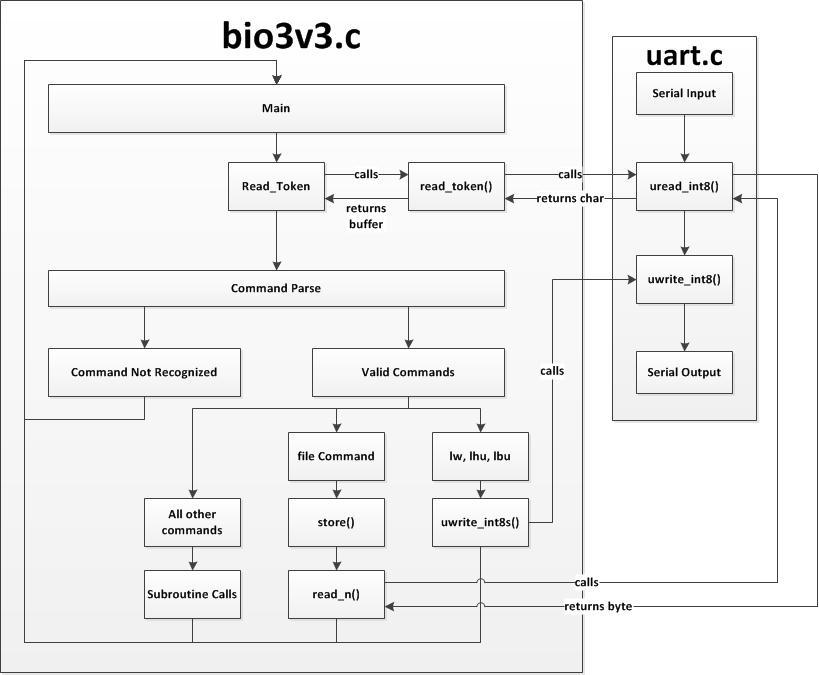
\includegraphics[width=0.7\textwidth]{bios_flow.png}
  \caption{BIOS Execution Flow}
\end{figure}

The buffer returned from the \verb|read_token| method with the user input is then parsed by
comparing the returned buffer against commands that the BIOS recognizes. If the BIOS parses a
command successfully it will execute the appropriate subroutine or commands. Otherwise it
will tell you that the command you input is not recognized.
If you want to add commands to the BIOS at any time in the project, you will have to add to the
comparisons that follow after the \verb|read_token| subroutine in the BIOS.

\subsection{The UART}
You will notice that some of the BIOS execution calls will call subroutines in the uart.c file
which takes care of the transmission and reception of byte over the serial line.
The uart.c file contains three subroutines. The first subroutine, \verb|uwrite_int8| executes a
UART transmission for a single byte by writing to the output data register. The second
subroutine \verb|uwrite_int8s| allows you to process an array of type \verb|int8_t| or chars and send
them over the serial line. The third routine \verb|uread_int8| polls the UART for valid data and
reads a byte from the serial line.

In essence, these three routines are operating the UART on your design from a software view
using the memory mapped I/O. Therefore, in order for the software to operate the memory
map correctly, the \verb|uart.c| module must store and load from the correct addresses as defined
by out memory map. You will find the necessary memory map addresses in the uart.h file that
conforms to the design specification.

\subsection{Command List}
The following commands are built into the BIOS that we provide for you. All values are
interpreted in hexadecimal and do not require any radix prefix (ex. ``0x''). Note that there is not
backspace command.

\verb|jal <hexadecimal address>| - Moves program execution to the specified address

\verb|lw <hexadecimal address>| - Displays word at specified address to screen

\verb|lhu <hexadecimal address>| - Displays half at specified address to screen

\verb|lbu <hexadecimal address>| - Displays byte at specified address to screen

\verb|sw <value> <hexadecimal address>| - Stores specified word to address in memory

\verb|sh <value> <hexadecimal address>| - Stores specified half to address in memory

\verb|sb <value> <hexadecimal address>| - Stores specified byte to address in memory

There is another command file in the main() method that is used only when you execute
\verb|hex_to_serial|. When you execute \verb|hex_to_serial|, your workstation will initiate a byte
transfer by calling this command in the BIOS. Therefore, don’t mess with this command too
much as it is one of the more critical components of your BIOS.

\subsection{Adding Your Own Features}
Feel free to modify the BIOS code if you want to add your own features during the project for
fun or to make your life easier. If you do choose to modify the BIOS, make sure to preserve
essential functionality such as the I/O and the ability to store programs. In order to add
features, you can either add to the code in the \verb|bios151v3.c| file or create your own c source and
header files. Note that you do not have access to standard c libraries so you will have to add
them yourself if you need additional library functionality.
\end{document}

% ARCHIVE
%\subsubsection{Music Streamer in Software}
%Now that we have access to user I/Os and access to the tone generator, we can fully implement the music streamer and sequencer FSM from lab 4 entirely in software!
%
%The music streamer program can be found in \verb|software/music_streamer|. To use this program, use the same scripts from Lab 3 to generate a music data file from a MusicXML file, and then convert that data file to a static array declaration that can be used in a C program.
%
%\begin{minted}[frame=single]{bash}
%python scripts/musicxml_parser.py musicxml/Row_Row_Row_Your_Boat.mxl music.txt
%\end{minted}
%
%You will now have a \verb|music.txt| file in the \verb|/software/music_streamer| directory with the music data. Now we use the \verb|c_array_generator.py| script to create a static array declaration using this file.
%
%\begin{minted}[frame=single]{bash}
%python scripts/c_array_generator.py music.h music.txt
%\end{minted}
%
%Now, we have a file called \verb|music.h| that has a static array declaration filled with the music data. This serves exactly the same purpose as the ROM that was generated in Lab 3.
%
%To build the \verb|music_streamer| program and place it on your processor, execute:
%\begin{minted}[frame=single]{bash}
%make
%hex_to_serial music_streamer.hex 3000a000
%screen $SERIALTTY 115200
%151> jal 1000a000
%\end{minted}
%
%The \verb|music_streamer| functions exactly like it does in Lab 3, but the state machine that was implemented directly in hardware, is now implemented in software. Here is the state machine diagram for reference:
%
%\begin{center}
%  \begin{tikzpicture}[shorten >=1pt, node distance=10cm,on grid, auto, semithick]
%  \tikzstyle{state} = [draw, very thick, fill=white, rectangle, minimum height=3em, minimum width=7em, node distance=12em, font={\sffamily\bfseries}]
%  \tikzstyle{stateEdgePortion} = [black,thick];
%  \tikzstyle{stateEdge} = [stateEdgePortion,->];
%  \tikzstyle{edgeLabel} = [pos=0.5, text centered, font={\sffamily\small}];
%
%  \node[state,initial](rp) {REGULAR\_PLAY};
%  \node[state](revp) [below =of rp]{REVERSE\_PLAY};
%  \node[state](p) [right=of rp]{PAUSED};
%  \node[state](playseq) [above=of rp]{PLAY\_SEQ};
%  \node[state](editseq) [left=of rp]{EDIT\_SEQ};
%
%  \path[->]
%  (playseq) edge node [swap] {play\_pause} (p)
%  edge node [swap] {switch\_mode} (editseq)
%  edge node {} (rp)
%  (editseq) edge node {} (playseq)
%  (rp) edge node {play\_pause} (p)
%  edge [swap] node {switch\_mode} (revp)
%  edge node {switch\_fn} (playseq)
%  (p) edge node {} (rp)
%  edge [bend right, swap] node {switch\_fn} (playseq)
%  (revp) edge [swap] node {play\_pause} (p)
%  edge [swap] node {} (rp);
%  \end{tikzpicture}
%\end{center}
%
%The program will print out information as you transition the state machine, edit notes in the sequencer, and modify the tempo.
